
%% add 'handout' option for handouts, and pgfpages for 2-on-1
%\documentclass[smaller,compress]{beamer}   
\documentclass[compress]{beamer}   
  
%\usepackage{pgfpages}
%\pgfpagesuselayout{2 on 1}[letterpaper,border shrink=5mm]
%\pgfpagesuselayout{4 on 1}[letterpaper,border shrink=5mm]
%\pgfpagesuselayout{2 on 1}[a4,border shrink=5mm]

\usepackage{color}

\mode<presentation>
{
  %\usetheme[secheader]{Madrid} % nice (once my coloroverrides are sorted out)
  %\usetheme{AnnArbor}	% nice!	
  %\usetheme{Malmoe}	% nice!	
  \usetheme{Warsaw}	% nice!	

  %\usetheme[secheader]{Boadilla} % ok
  %\usecolortheme{whale}
  %\usecolortheme{orchid}
}

% Delete this, if you do not want the table of contents to pop up at
% the beginning of each subsection (or section)
% edd: Does not work in handout mode, and we have too many section/subsections
\AtBeginSection[]{%
  \begin{frame}<beamer>%
    %\tiny
    \frametitle{Outline}%
    \tableofcontents[currentsection]
  \end{frame}
}


% If you wish to uncover everything in a step-wise fashion, uncomment the following command: 
%\beamerdefaultoverlayspecification{<+->}

\newcommand{\MedSkip}{\medskip \par} % add \pause if desired 
\newcommand{\SmallSkip}{\smallskip} % add \pause if desired 

\usepackage[english]{babel}   	% or whatever
\usepackage[latin1]{inputenc}	% or whatever
\usepackage{times}
\usepackage[T1]{fontenc}		% Or whatever. Note that the encoding and the 
								% font should match. If T1 does not look
                                % nice, try deleting the line with the fontenc.
\usepackage{highlight}
\usepackage{color}
\usepackage{alltt}

% \usepackage{animate}

\usepackage{listings}
\lstset{ %
  language=R,                   % choose the language of the code
  basicstyle=\scriptsize,       % the size of the fonts that are used for the code
  numbers=left,                 % where to put the line-numbers
  numberstyle=\tiny,            % the size of the fonts that are used for the line-numbers
  stepnumber=1,                 % the step between two line-numbers. If it's 1 each line will be numbered
  numbersep=5pt,                % how far the line-numbers are from the code
  backgroundcolor=\color{white},% choose the background color. You must add \usepackage{color}
  showspaces=false,             % show spaces adding particular underscores
  showstringspaces=false,       % underline spaces within strings
  showtabs=false,               % show tabs within strings adding particular underscores
  frame=single,                 % adds a frame around the code
  tabsize=2,                    % sets default tabsize to 2 spaces
  captionpos=b,                 % sets the caption-position to bottom
  breaklines=true,              % sets automatic line breaking
  breakatwhitespace=false,      % sets if automatic breaks should only happen at whitespace
  escapeinside={\%*}{*)}        % if you want to add a comment within your code
}

\hypersetup{                  		% beamer colors taken from elsewhere
  hyperindex,%				% works with the beetle colour scheme
  colorlinks,%
  linktocpage,%
  plainpages=true,%
  linkcolor=myOrange,%
  citecolor=myDarkGrey,%
  urlcolor=myDarkBlue,%
  pdfstartview=Fit,%
  pdfview={XYZ null null null}%
}
%\hypersetup{                  		% beamer colors taken from elsewhere
%  hyperindex,%				% works with the beetle colour scheme
%  colorlinks%
%  linktocpage,%
%  plainpages=false,%
%  linkcolor=eddBlue,%
%  citecolor=eddDarkGrey,%
%  urlcolor=eddDarkBlue,%
%  pdfstartview=Fit,%
%  pdfview={XYZ null null null}%
%}

\RequirePackage{color}
\definecolor{Red}{rgb}{0.7,0,0}
\definecolor{myOrange}{rgb}{0.8,0.5,0.0}
\definecolor{myBlue}{rgb}{0.0,0.0,0.4}
\definecolor{myDarkBlue}{rgb}{0.1,0.1,0.4}
\definecolor{myDarkGrey}{rgb}{0.15,0.15,0.15}
% Doug's
\definecolor{Sinput}{rgb}{0,0,0.56}
\definecolor{Scode}{rgb}{0,0,0.56}
\definecolor{Soutput}{rgb}{0.56,0,0}
% 
\definecolor{Cmdinput}{rgb}{0,0,0.44}
\definecolor{Cmdoutput}{rgb}{0.44,0,0}
\definecolor{Cppinput}{rgb}{0.15,0.15,0.15}

%% based on Doug's, but mod'ed \R to use hyperref
\RequirePackage{fancyvrb}
\RequirePackage{xspace}
\RequirePackage{paralist}
\newenvironment{Schunk}{\par\begin{minipage}{\textwidth}}{\end{minipage}}
\DefineVerbatimEnvironment{Sinput}{Verbatim}{formatcom={\color{Sinput}},fontsize=\small}
\DefineVerbatimEnvironment{Soutput}{Verbatim}{formatcom={\color{Soutput}},fontsize=\footnotesize}
\DefineVerbatimEnvironment{Scode}{Verbatim}{formatcom={\color{Scode}},fontsize=\small}
\DefineVerbatimEnvironment{Cmdinput}{Verbatim}{formatcom={\color{Cmdinput}},fontsize=\small}
\DefineVerbatimEnvironment{Cmdoutput}{Verbatim}{formatcom={\color{Cmdoutput}},fontsize=\footnotesize}
\DefineVerbatimEnvironment{Cppinput}{Verbatim}{formatcom={\color{Cppinput}},fontsize=\small}

% -- not \small 
\newcommand{\smallcode}[1]{{\color{Sinput}\small\texttt{#1}}}
\newcommand{\code}[1]{{\color{Sinput}\texttt{#1}}}
\newcommand{\Emph}[1]{\emph{\color{Scode}#1}}   
%\newcommand{\R}{\href{http://www.r-project.org}{\Emph{R}\xspace}}   %% ? sing \emph upsets beamer inside \href
\newcommand{\R}{\href{http://www.r-project.org}{\textsf{R}\xspace}}
\newcommand{\Rns}{\href{http://www.r-project.org}{\textsf{R}}}

\newcommand{\QL}{\href{http://www.QuantLib.org}{\textsf{QuantLib}\xspace}}
\newcommand{\pkg}[1]{\textbf{#1}}
% two old defintions
%\newcommand{\code}[1]{\texttt{#1}}
\newcommand{\screenshot}[1]{\centerline{\includegraphics[height=7.8cm,transparent]{#1}}}  % 7.8in


% If you have a file called "university-logo-filename.xxx", where xxx
% is a graphic format that can be processed by latex or pdflatex,
% resp., then you can add a logo as follows:
% NB transparent in Adobe but not in kpdf
%\pgfdeclareimage[height=0.6cm]{useR-logo}{figures/useR}
%\logo{\pgfuseimage{useR-logo}}

  %% has all definitions etc

\title[RQuantLib]{RQuantLib: Interfacing QuantLib from R}  %% better title welcome...
\subtitle{\textsl{R / Finance 2010 Presentation}}
\subject{R / Finance 2010 Presentation}
\author[Eddelbuettel \and Nguyen]{Dirk Eddelbuettel\inst{1} \and Khanh Nguyen\inst{2}}
\institute[Debian and UMASS]{
  \inst{1}%
  Debian Project
  \and 
  \inst{2}
  UMASS at Boston
} 
\date[R / Finance 2010]{R / Finance 2010 \\ April 16 and 17, 2010 \\ Chicago, IL, USA}

\begin{document}

\begin{frame}
  \titlepage
\end{frame}

% \section{Introduction (draft, just an idea)}
% \begin{frame}
%   \frametitle{Overview}
%   \framesubtitle{Presentation details}
%   \begin{itemize}
% \small
%   \item Brief overview of QuantLib
%     \begin{itemize}
%     \item History, about to release 1.0 after eight long years
%     \item Luigi's design document draft, mention rigorous design, unit
%       tests, boost, 'grown up C++'
%     \item Maybe mention different language bindings
%     \item Maybe mention liberal QL license; R / RQuantLib with GPL somewhat
%       tighter but in spirit of R community
%     \end{itemize}
%   \item RQuantLib maybe chronologically
%     \begin{itemize}
%     \item Equity options part
%     \item Simple calendaring
%     \item Mention the older fixed income / curve stuff without dwelling on it
%     \end{itemize}
%   \item Fixed Income / GSoC 2009
%     \begin{itemize}
%     \item Khanh ....
%     \item More Khanh ...
%     \end{itemize}
%   \item Total of somewhere between 20 and 30 pages
%   \item Finish with Outlook / Agenda / Areas not yet covered
%   \end{itemize}
% \end{frame}

\section{QuantLib}
\subsection{Overview}
\begin{frame}
  \frametitle{A brief introduction to QuantLib}
  \framesubtitle{What is it, and who wrote is behind it?}
  \begin{columns}
    \begin{column}{1.5in}
      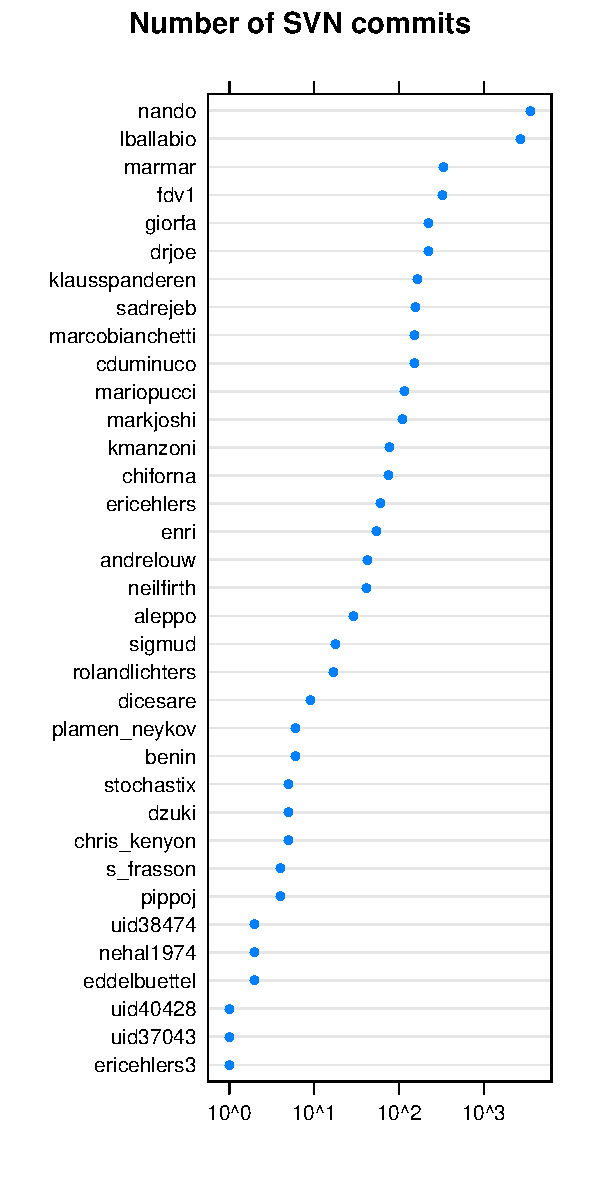
\includegraphics[width=1.5in]{figures/ql-svn.pdf}
    \end{column}
    
    \begin{column}{3.1in}
      \begin{itemize}
      \item \QL is a C++ library for financial quantitative analysts and developers.
      \item \QL was started in 2000 and is hosted on Sourceforge.Net
      \item \QL is a free software project under a very liberal license allowing
        for inclusion in commercial projects.
      \item \QL is primarily the work of Ferdinando Ametrano and Luigi Ballabio.
        %with a supporting cast of other contributors. 
      \item \QL is sponsored by the Italian consultancy StatPro which derives
        consulting income from it. 
      \end{itemize}
    \end{column}
  \end{columns}
\end{frame}


\subsection{Timeline}
\begin{frame}
  \frametitle{QuantLib releases}
  \framesubtitle{Showing the growth of QuantLib over time}

  \begin{columns}
    % \begin{column}{1.25in}
    %   \scriptsize
    %   \begin{tabular}{lrl}
    %     % \toprule
    %     Version & Date &\\ 
    %     % \midrule
    %     1.0   & 24 Feb 2010 & \\
    %     0.9.9 & 11 Nov 2009 & \\
    %     0.9.7 & 18 Nov 2008 & \\
    %     0.9.6 & 06 Aug 2008 & \\
    %     0.9.5 & 30 Jul 2008 & \\
    %     0.9.0 & 24 Dec 2007 & \\
    %     0.8.1 & 04 Jun 2007 & \\
    %     0.8.0 & 30 May 2007 & \\
    %     0.4.0 & 20 Feb 2007 & \\
    %     0.3.14& 06 Nov 2006 & \\
    %     0.3.13& 31 Jul 2006 & \\
    %     0.3.12& 27 Mar 2006 & \\
    %     0.3.11& 20 Oct 2005 & \\
    %     \phantom{X} & & 
    %   \end{tabular}
    % \end{column}

    % \begin{column}{0.25in}
    %   \phantom{XX}  % empty, not shown
    % \end{column}

    % \begin{column}{2.75in}
    %   \scriptsize
    %   \begin{tabular}{lrl}
    %     % \toprule
    %     Version & Date &\\ 
    %     % \midrule
    %     0.3.10& 14 Jul 2005 & \\
    %     0.3.9 & 02 May 2005 & \\
    %     0.3.8 & 22 Dec 2004 & \\
    %     0.3.7 & 23 Jul 2004 & 1st \QL with Boost \\
    %     0.3.6 & 15 Apr 2004 & \\
    %     0.3.5 & 31 Mar 2004 & \\
    %     0.3.4 & 12 Nov 2003 & \\
    %     0.3.3 & 03 Sep 2003 & \\
    %     0.3.1 & 04 Feb 2003 & \\
    %     0.3.0 & 06 May 2002 & \\
    %     0.2.1 & 03 Dec 2001 & (first RQuantLib Feb 2002) \\
    %     0.2.0 & 18 Sep 2001 & \\
    %     0.1.9 & 31 May 2001 & 1st \QL Debian package \\
    %     0.1.1 & 21 Nov 2000 & \\
    %   \end{tabular}
    % \end{column}

    \begin{column}{2.9in}
      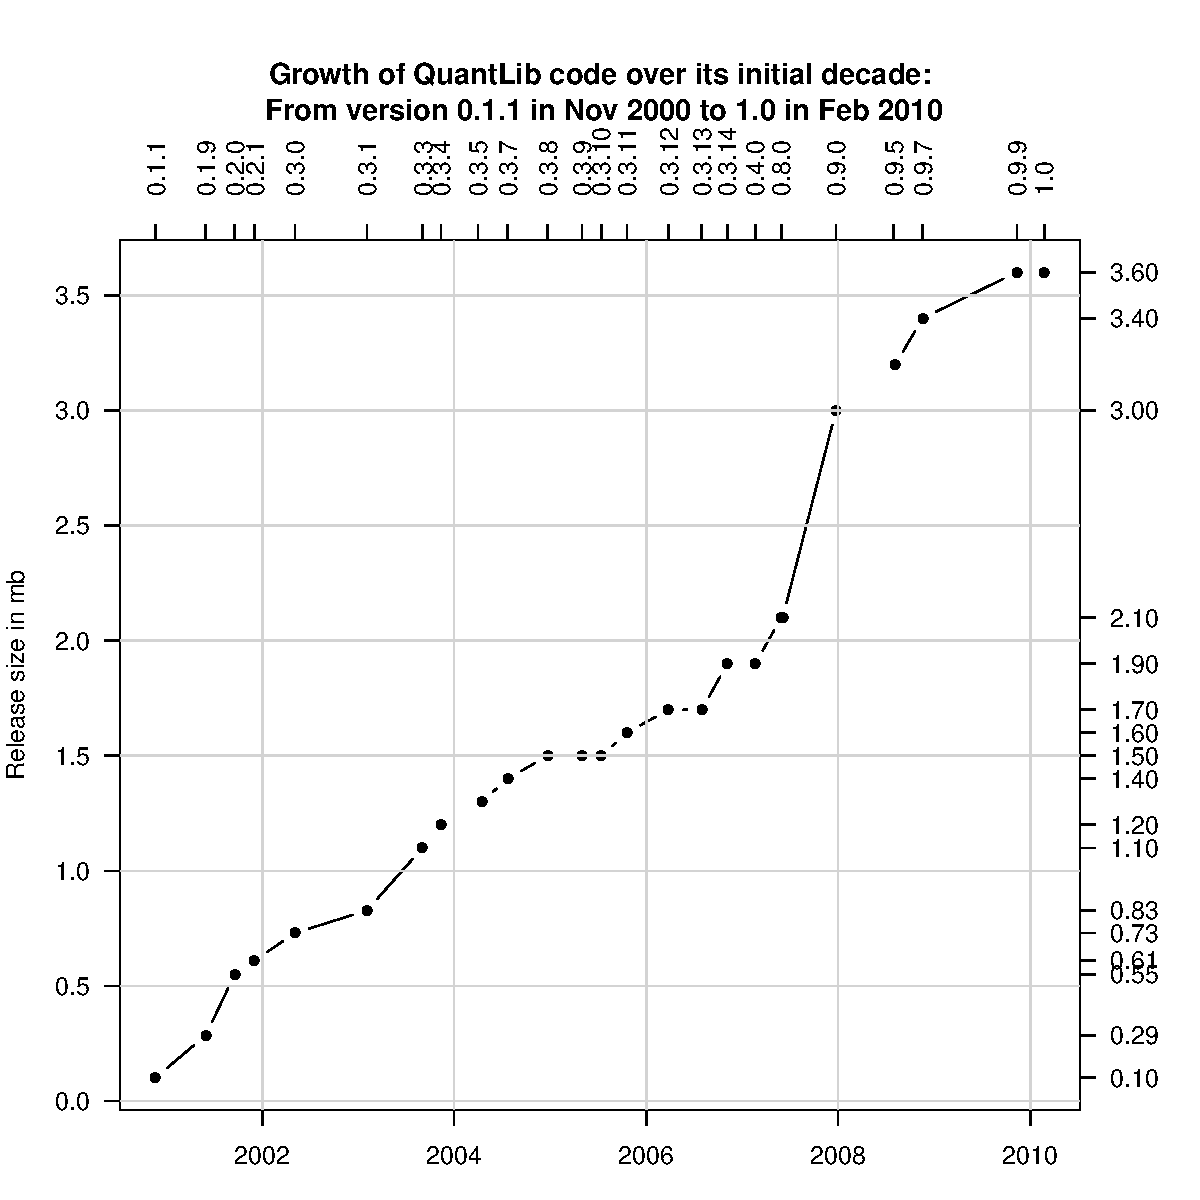
\includegraphics[height=2.9in]{figures/qlReleases.pdf}
    \end{column}
    
    \begin{column}{2in}
      \begin{itemize}
      \item The initial release was 0.1.1 in Nov 2000
      \item The first Debian package was prepared in May 2001
      \item Boost has been a requirement since July 2004
      \item The long awaited 1.0.0 release appeared in Feb 2010
      \end{itemize}
    \end{column}
  \end{columns}
\end{frame}

\subsection{Architecture}
\begin{frame}
  \frametitle{QuantLib Architecture}
  \framesubtitle{How is it put togetherm and how do I use it?}
  \begin{itemize}
  \item \QL is written in C++ and fairly rigourously designed. 
  \item Luigi Ballabio has draft chapters on the \QL design and
    implementation at \url{http://sites.google.com/site/luigiballabio/qlbook}.
  \item \QL use the Boost testing framework and employs hundreds
    of detailed unit tests. 
  \item \QL makes extensive use of Swig and bindings for Java, Perl, 
    Python, Ruby, C\#, Guile ... exist. 
  \item QuantLibAddin exports a procedural interface to a number of platforms
    including Excel and Oo Calc.
  \item Several \textsl{manual} (non-SWIG) extension such as \pkg{RQuantLib}
    exist as well.
  \end{itemize}
\end{frame}

\begin{frame}
  \frametitle{Key Modules}
  \framesubtitle{A rough guide, slight re-arranged from the QuantLib documentation}
  \begin{itemize}
  \item Currencies and FX rates
  \item Date and time calculations (Calendars, Day Counters)
  \item Pricing engines (Asian, Barrier, Basket, Cap/Floor, Cliquet, Forward, Quanto,
    Swaption, Vanilla)
  \item Finite-differences framework
  \item Fixed-Income (Short-rate modelling, Term structures)
  \item Financial instruments
  \item Math tools (Lattice method, Monte Carlo Framework, Stochastic Process)
  \item Utilities (Numeric types, Design patterns, Output manipulators)
  \item QuantLib macros (Numeric limits, Debugging)
  \end{itemize}
\end{frame}

\subsection{Examples}
\begin{frame}[fragile]
  \frametitle{Options: Fifteen solutions and three different exercises}
\tiny
  \begin{verbatim}
$ EquityOption

Option type = Put
Maturity = May 17th, 1999
Underlying price = 36
Strike = 40
Risk-free interest rate = 6.000000 %
Dividend yield = 0.000000 %
Volatility = 20.000000 %


Method                             European      Bermudan      American
Black-Scholes                      3.844308      N/A           N/A
Barone-Adesi/Whaley                N/A           N/A           4.459628
Bjerksund/Stensland                N/A           N/A           4.453064
Integral                           3.844309      N/A           N/A
Finite differences                 3.844342      4.360807      4.486118
Binomial Jarrow-Rudd               3.844132      4.361174      4.486552
Binomial Cox-Ross-Rubinstein       3.843504      4.360861      4.486415
Additive equiprobabilities         3.836911      4.354455      4.480097
Binomial Trigeorgis                3.843557      4.360909      4.486461
Binomial Tian                      3.844171      4.361176      4.486413
Binomial Leisen-Reimer             3.844308      4.360713      4.486076
Binomial Joshi                     3.844308      4.360713      4.486076
MC (crude)                         3.834522      N/A           N/A
QMC (Sobol)                        3.844613      N/A           N/A
MC (Longstaff Schwartz)            N/A           N/A           4.481675

Run completed in 5 s

  \end{verbatim}
\end{frame}

\begin{frame}[fragile]
  \frametitle{Errors from discrete hedging (Derman and Kamal)}
{ \tiny
  \begin{verbatim}
$ DiscreteHedging

Option value: 2.51207

         |          |      P&L |      P&L | Derman&Kamal |      P&L |      P&L
 samples |   trades |     mean | std.dev. |      formula | skewness | kurtosis
------------------------------------------------------------------------------
   50000 |       21 |   -0.001 |     0.43 |         0.44 |    -0.33 |     1.56
   50000 |       84 |    0.000 |     0.22 |         0.22 |    -0.20 |     1.68

Run completed in 16 s
  \end{verbatim}
}

Other examples include \texttt{SwapValuation}, \texttt{Repo},
\texttt{Replication}, \texttt{FRA}, \texttt{FittedBondCurve}, \texttt{Bonds},
\texttt{BermudanSwaption}, \texttt{CDS}, \texttt{ConvertibleBonds},
\texttt{CallableBonds} and \texttt{MarketModels}

\end{frame}

\section{RQuantLib}
\subsection{Overview}
\subsection{Key components}
\begin{frame}
  \frametitle{Overview}
  \begin{itemize}
  \item Initial implementation: Standard equity option pricing:
    \begin{itemize}
      \item pricers and greeks for European and American options
      \item first set of exotics using barrier and binaries
      \item also implied volatility calculations where available
    \end{itemize}
  \item First external contribution: Curves and Swaption pricing.
  \item Second external contribution (as Google Summer of Code): Fixed Income
    Functionality (more on this below)
  \item Other small extensions on date and holiday calculations.
  \end{itemize}
\end{frame}


\section{Fixed Income}
\subsection{Overview and development}

\begin{frame}
	\frametitle{Fixed Income Development}
	RQuantLib before GSOC 2009...
	\begin{center}
		\resizebox{95mm}{!}{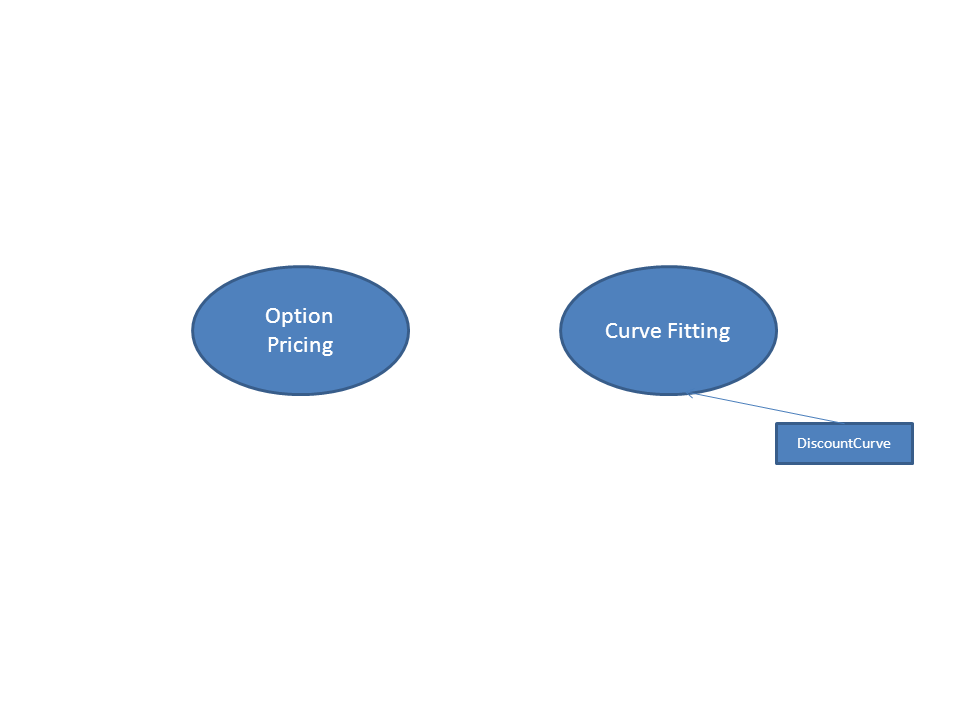
\includegraphics{figures/fixedIncomeDev/Slide1.PNG}}
	\end{center}
\end{frame}
\begin{frame}
	\frametitle{Fixed Income Development}
	GSOC started. April 2009...
	\begin{center}
		\resizebox{95mm}{!}{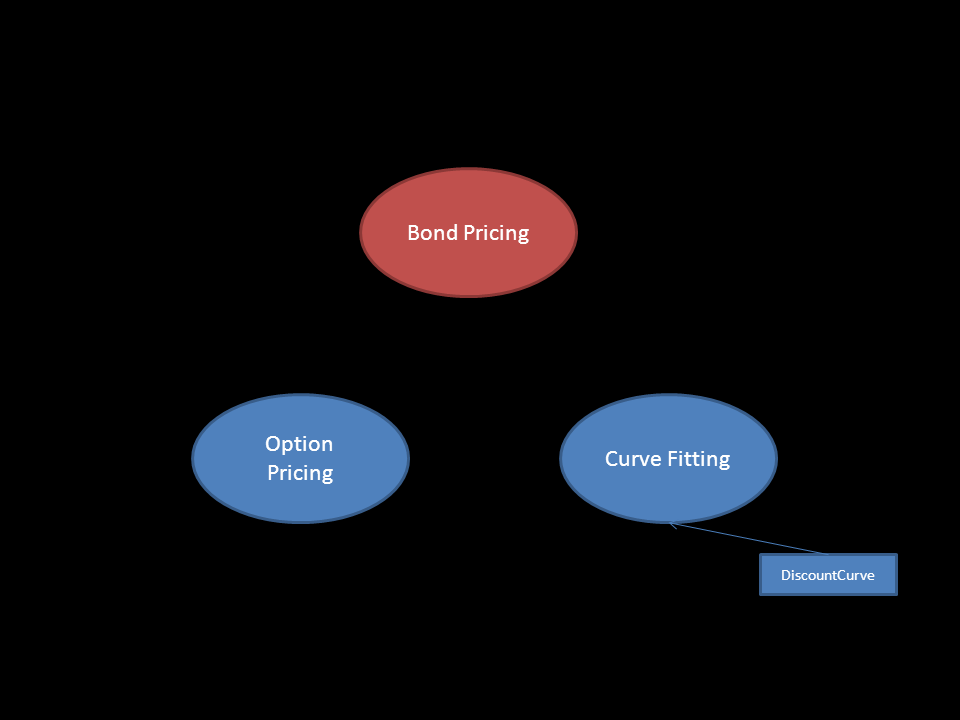
\includegraphics{figures/fixedIncomeDev/Slide2.PNG}}
	\end{center}
\end{frame}
\begin{frame}
	\frametitle{Fixed Income Development}

	\begin{center}
		\resizebox{95mm}{!}{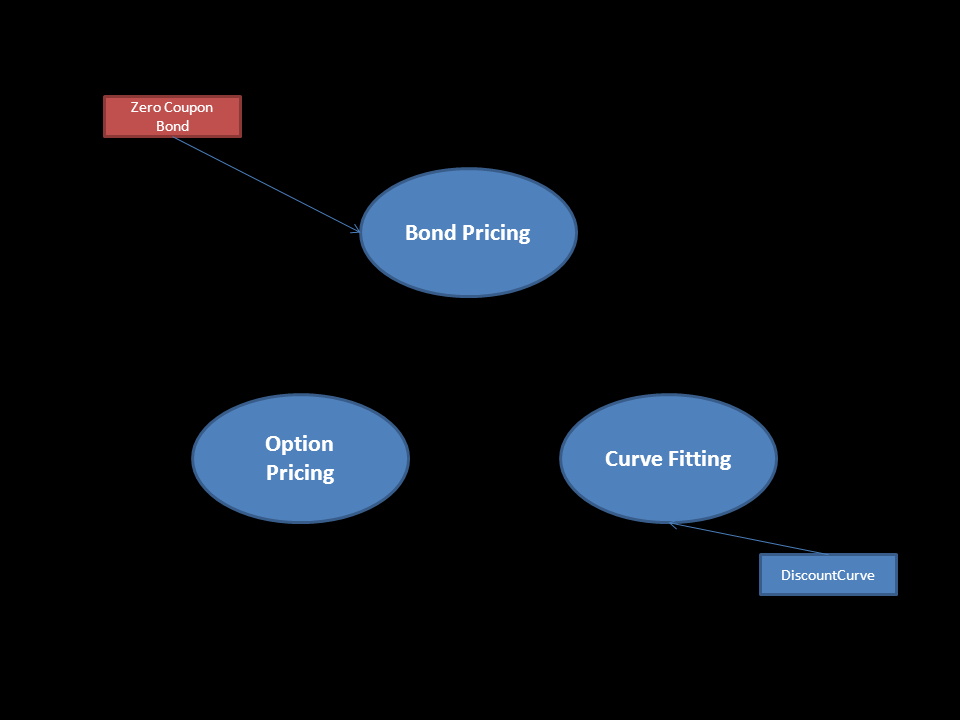
\includegraphics{figures/fixedIncomeDev/Slide3.PNG}}
	\end{center}
\end{frame}
\begin{frame}
	\frametitle{Fixed Income Development}
	\textcolor{white}{}
	\begin{center}
		\resizebox{95mm}{!}{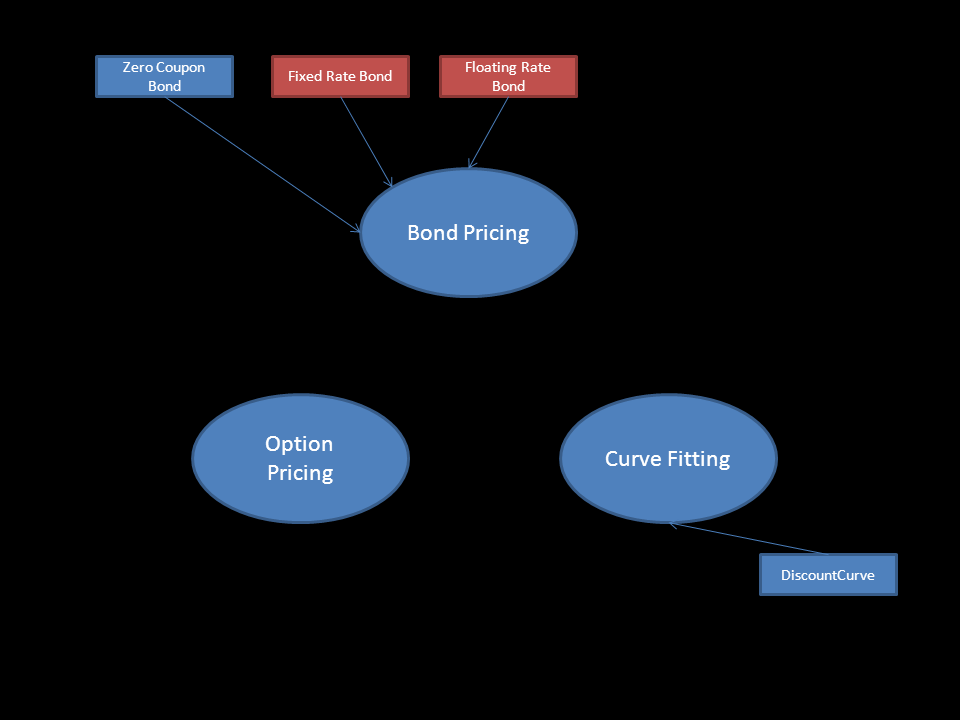
\includegraphics{figures/fixedIncomeDev/Slide4.PNG}}
	\end{center}
\end{frame}
\begin{frame}
	\frametitle{Fixed Income Development}
	Making curve fitting and bond pricing work together...
	\begin{center}
		\resizebox{95mm}{!}{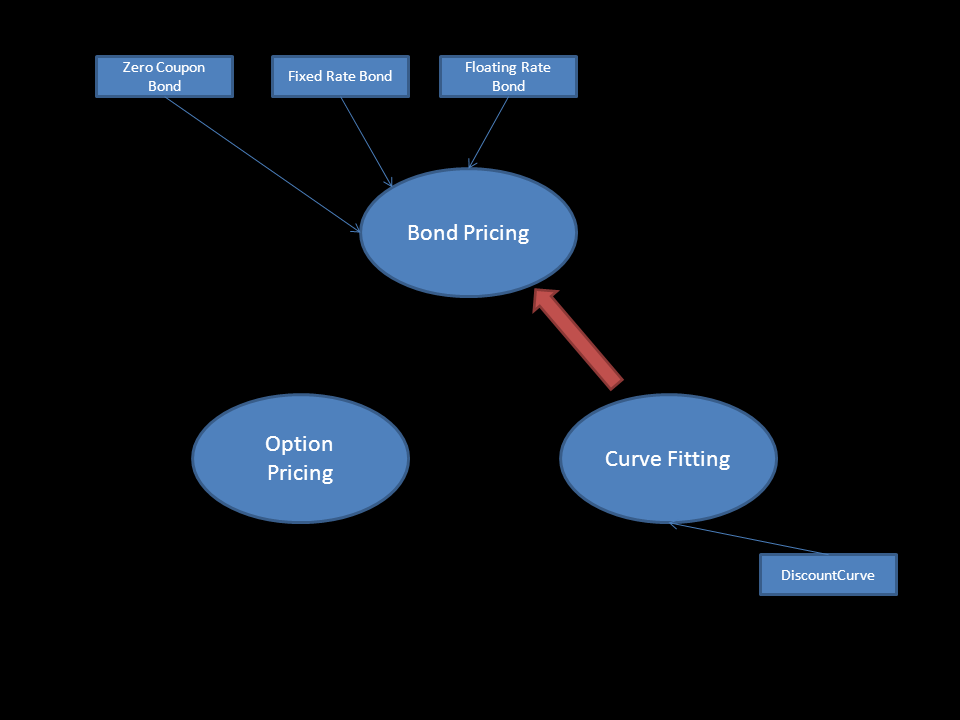
\includegraphics{figures/fixedIncomeDev/Slide5.PNG}}
	\end{center}
\end{frame}
\begin{frame}
	\frametitle{Fixed Income Development}

	\begin{center}
		\resizebox{95mm}{!}{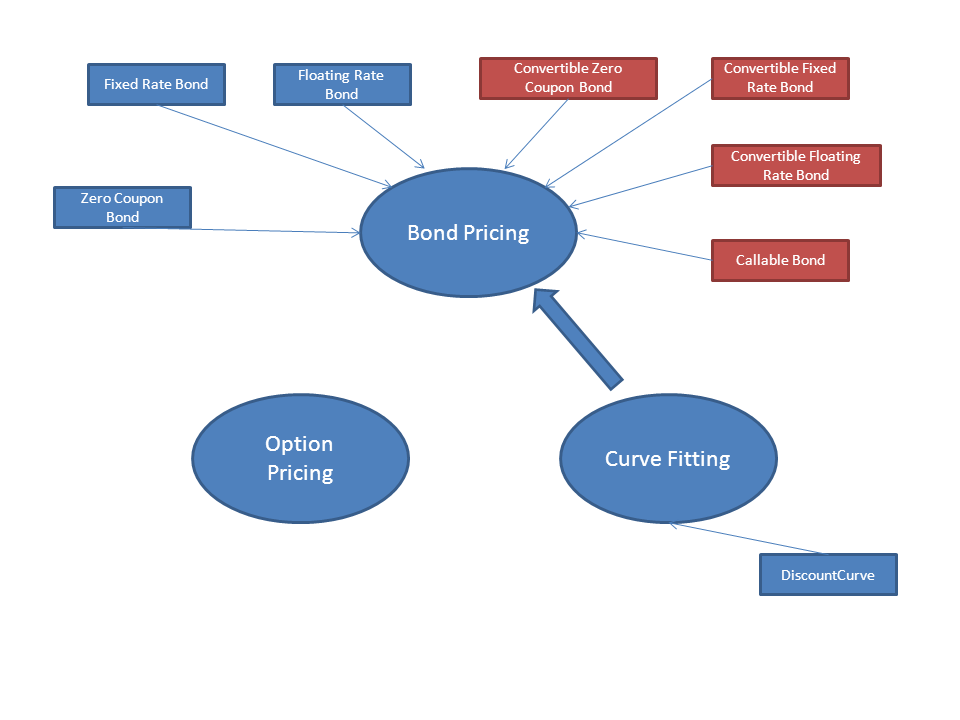
\includegraphics{figures/fixedIncomeDev/Slide6.PNG}}
	\end{center}
\end{frame}
\begin{frame}
	\frametitle{Fixed Income Development}
	\begin{center}
		\resizebox{95mm}{!}{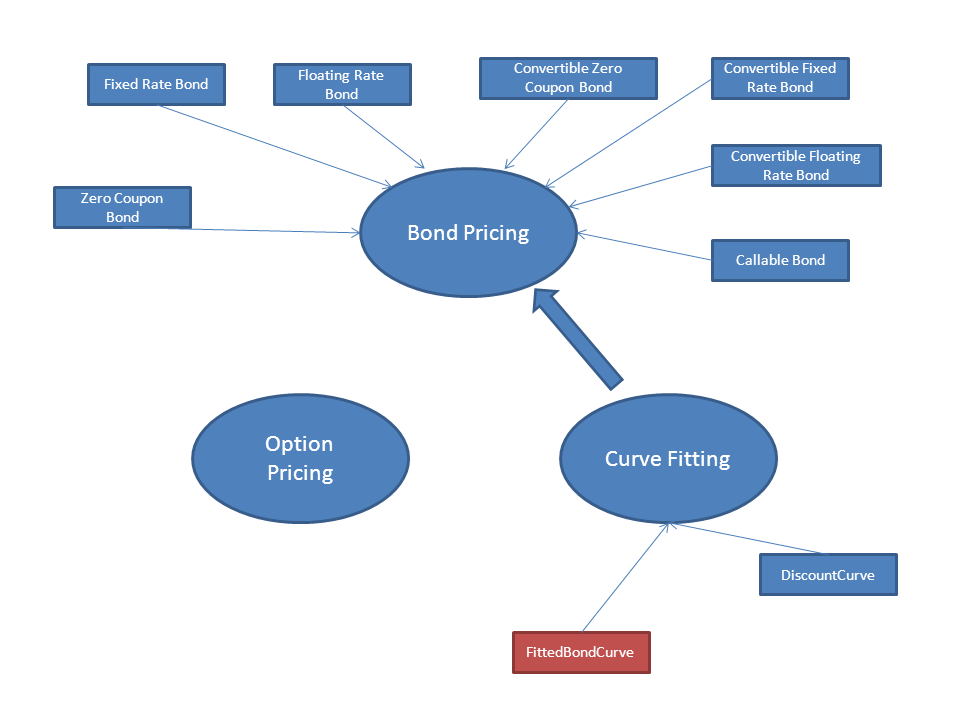
\includegraphics{figures/fixedIncomeDev/Slide7.PNG}}
	\end{center}
\end{frame}
\begin{frame}
	\frametitle{Fixed Income Development}
	And recently, we have a \textcolor{red}{GUI}
	\begin{center}
		\resizebox{95mm}{!}{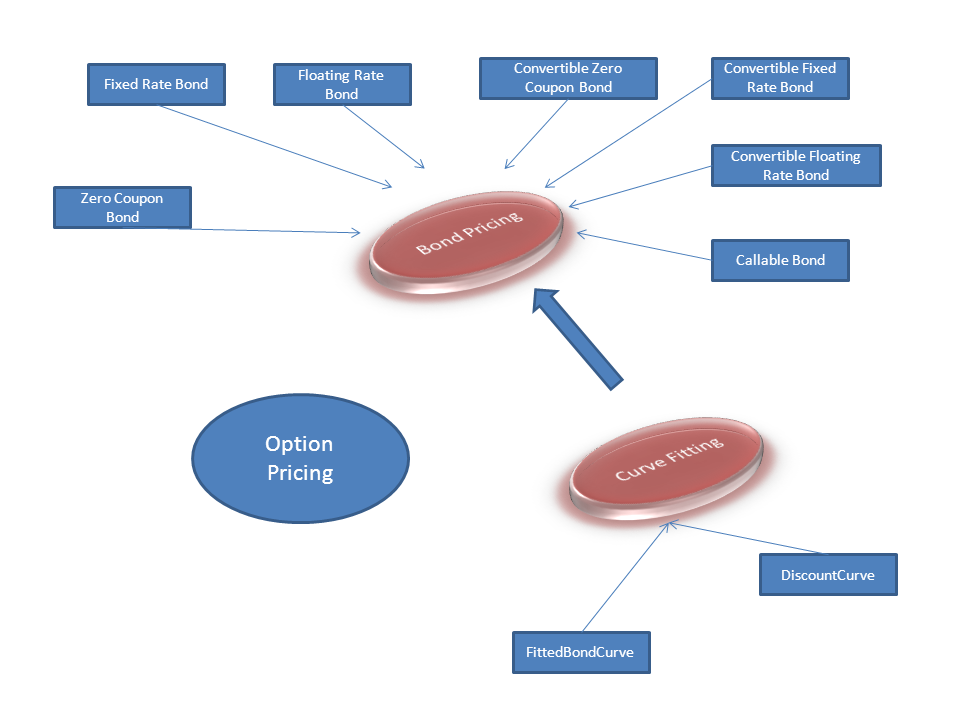
\includegraphics{figures/fixedIncomeDev/Slide8.PNG}}
	\end{center}
\end{frame}
\begin{frame}
	\frametitle{Fixed Income Development}
	\begin{center}\huge In summary\end{center}
	\begin{center}
		\resizebox{95mm}{!}{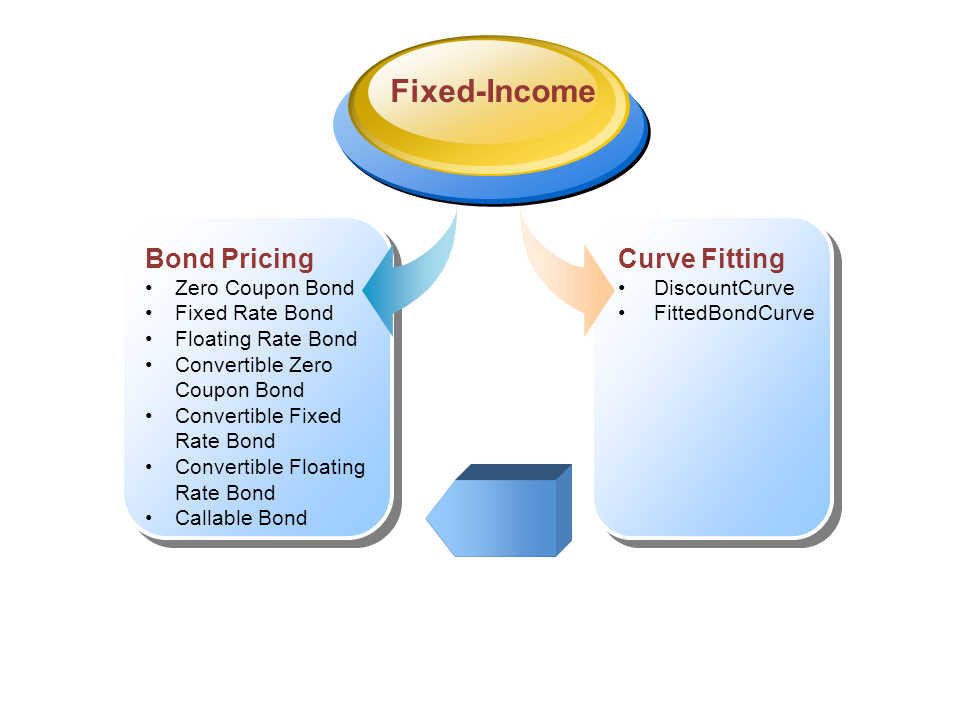
\includegraphics{figures/fixedIncomeDev/Slide9.png}}
	\end{center}

\end{frame}

%
%\begin{frame}
%	\frametitle{Fixed Income in RQuantLib}
%	In summary,
%	\begin{itemize}
%		\item Fixed Income functions are added during the summer of 2009 as part of the Google Summer of Code program. 
%		\item  RQuantLib offeres strong support for fixed income pricing whereas several other packages (e.g. termstrc, YieldCurve, fBonds) focus on modelling term structure.		
%		\item The functions aim to support two primary tasks: pricing and curve fitting. 		
%	\end{itemize}
%\end{frame}
%
%
%\begin{frame}
%	\frametitle{Fixed Income in RQuantLib}
%	\framesubtitle{Primary tasks: Curve fitting}
%	\begin{itemize}
%		\item Curve fitting functions
%			\begin{itemize}
%				\item Curve fitting functions return a DiscountCurve object that contains a two column dates/zeroRates data frame.
%				\item The returned DiscountCurve object are used as inputs for pricing functions. 
%			\end{itemize}
%		\item Currently, there are two curve fitting functions
%			\begin{itemize}
%				\item DiscountCurve - constructs the spot term structure of interest rates based on input market data including the settltment date, deposit rates, future prices, FRA rates or swap rates in various combination.
%				\item FittedBondCurve - fits a term structure to a set of bonds using three different fitting methods (ExponentialSplinesFitting, SimplePolynomialFitting, NelsonSiegelFitting).
%			\end{itemize}
%	\end{itemize}
%\end{frame}
%
%\begin{frame}
%	\frametitle{Fixed Income in RQuantLib}
%	\framesubtitle{Primary tasks: Bond pricing}
%	\begin{itemize}
%		\item Bond pricing functions return clean price, dirty price, NPV and cash flow of a bond
%		\item Currently, the following bonds are supported
%			\begin{itemize}
%				\item Zero Coupon Bond
%				\item Fixed Rate Bond
%				\item Floating Rate Bond
%				\item Convertible Zero Coupon Bond
%				\item Convertible Fixed Rate Bond												
%				\item Convertible Floating Rate Bond
%				\item Callable Bond
%			\end{itemize}
%		\item The bonds available in QuantLib that yet are implemented are AmortizingCmsRateBond, AmortizingFixedRateBond, AmortizingFloatingRateBond, CallableFixedRateBond, CmsRateBond.
%	\end{itemize}
%\end{frame}

\subsection{Examples}
\begin{frame}[shrink]
	\frametitle{Fixed Income in RQuantLib}
	\framesubtitle{Examples: Curve fitting with DiscountCurve function}
Building a discount curve from the market data. This data is taken from codes shipped with QuantLib 0.9.7. 
\vskip15pt
\pagecolor{bgcolor}
\noindent
\scriptsize
\ttfamily
\hlstd{params\ }\hlsym{$<${-}\ }\hlstd{}\hlkwc{list}\hlstd{}\hlsym{(}\hlstd{tradeDate}\hlsym{=}\hlstd{}\hlkwc{as.Date}\hlstd{}\hlsym{(}\hlstd{}\hlstr{'2004{-}09{-}20'}\hlstd{}\hlsym{),}\hspace*{\fill}\\
\hlstd{}\hlstd{\ \ \ \ \ \ \ \ \ \ \ \ \ \ \ }\hlstd{settleDate}\hlsym{=}\hlstd{}\hlkwc{as.Date}\hlstd{}\hlsym{(}\hlstd{}\hlstr{'2004{-}09{-}22'}\hlstd{}\hlsym{),}\hspace*{\fill}\\
\hlstd{}\hlstd{\ \ \ \ \ \ \ \ \ \ \ \ \ \ \ }\hlstd{interpWhat}\hlsym{=}\hlstd{}\hlstr{"discount"}\hlstd{}\hlsym{,}\hspace*{\fill}\\
\hlstd{}\hlstd{\ \ \ \ \ \ \ \ \ \ \ \ \ \ \ }\hlstd{interpHow}\hlsym{=}\hlstd{}\hlstr{"loglinear"}\hlstd{}\hlsym{)}\hspace*{\fill}\\
\hlstd{tsQuotes\ }\hlsym{$<${-}\ }\hlstd{}\hlkwc{list}\hlstd{}\hlsym{(}\hlstd{d1w}\hlsym{=}\hlstd{}\hlnum{0.0382}\hlstd{}\hlsym{,\ }\hlstd{d1m}\hlsym{=}\hlstd{}\hlnum{0.0372}\hlstd{}\hlsym{,}\hspace*{\fill}\\
\hlstd{}\hlstd{\ \ \ \ \ \ \ \ \ \ \ \ \ \ \ \ \ }\hlstd{d3m}\hlsym{=}\hlstd{}\hlnum{0.0363}\hlstd{}\hlsym{,\ }\hlstd{d6m}\hlsym{=}\hlstd{}\hlnum{0.0353}\hlstd{}\hlsym{,}\hspace*{\fill}\\
\hlstd{}\hlstd{\ \ \ \ \ \ \ \ \ \ \ \ \ \ \ \ \ }\hlstd{d9m}\hlsym{=}\hlstd{}\hlnum{0.0348}\hlstd{}\hlsym{,\ }\hlstd{d1y}\hlsym{=}\hlstd{}\hlnum{0.0345}\hlstd{}\hlsym{,}\hspace*{\fill}\\
\hlstd{}\hlstd{\ \ \ \ \ \ \ \ \ \ \ \ \ \ \ \ \ }\hlstd{fut2}\hlsym{=}\hlstd{}\hlnum{96.7875}\hlstd{}\hlsym{,\ }\hlstd{fut3}\hlsym{=}\hlstd{}\hlnum{96.9875}\hlstd{}\hlsym{,}\hspace*{\fill}\\
\hlstd{}\hlstd{\ \ \ \ \ \ \ \ \ \ \ \ \ \ \ \ \ }\hlstd{fut4}\hlsym{=}\hlstd{}\hlnum{96.6875}\hlstd{}\hlsym{,\ }\hlstd{fut5}\hlsym{=}\hlstd{}\hlnum{96.4875}\hlstd{}\hlsym{,}\hspace*{\fill}\\
\hlstd{}\hlstd{\ \ \ \ \ \ \ \ \ \ \ \ \ \ \ \ \ }\hlstd{fut7}\hlsym{=}\hlstd{}\hlnum{96.2875}\hlstd{}\hlsym{,\ }\hlstd{s2y}\hlsym{=}\hlstd{}\hlnum{0.037125}\hlstd{}\hlsym{,}\hspace*{\fill}\\
\hlstd{}\hlstd{\ \ \ \ \ \ \ \ \ \ \ \ \ \ \ \ \ }\hlstd{s3y}\hlsym{=}\hlstd{}\hlnum{0.0398}\hlstd{}\hlsym{,\ }\hlstd{s5y}\hlsym{=}\hlstd{}\hlnum{0.0443}\hlstd{}\hlsym{,}\hspace*{\fill}\\
\hlstd{}\hlstd{\ \ \ \ \ \ \ \ \ \ \ \ \ \ \ \ \ }\hlstd{s10y}\hlsym{=}\hlstd{}\hlnum{0.05165}\hlstd{}\hlsym{,\ }\hlstd{s15y}\hlsym{=}\hlstd{}\hlnum{0.055175}\hlstd{}\hlsym{)}\hspace*{\fill}\\
\hlstd{curves\ }\hlsym{$<${-}\ }\hlstd{DiscountCurve}\hlsym{(}\hlstd{params}\hlsym{,\ }\hlstd{tsQuotes}\hlsym{)}\hlstd{}\hspace*{\fill}\\
\mbox{}
\normalfont
\end{frame}

\begin{frame}
	\frametitle{Fixed Income in RQuantLib}
	\framesubtitle{Examples: Curve fitting with DiscountCurve function}
\pagecolor{bgcolor}
\noindent
\scriptsize
\ttfamily
\hlstd{}\hlkwc{plot}\hlstd{}\hlsym{(}\hlstd{curves)}
\normalfont
\begin{center}
\resizebox{60mm}{!}{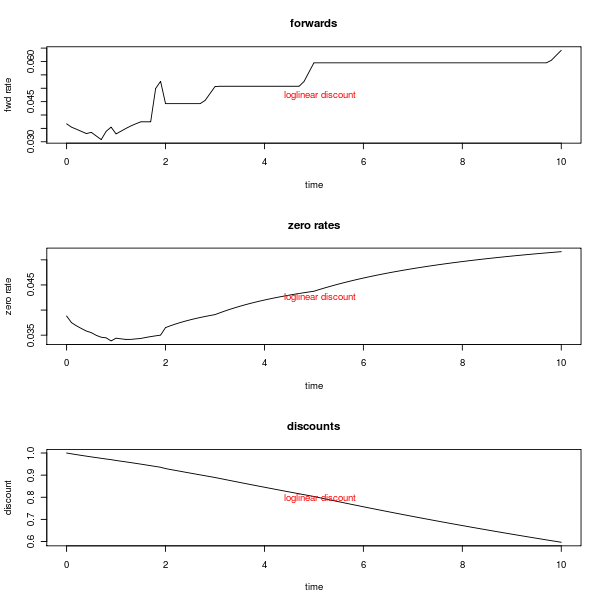
\includegraphics{figures/discountCurve.png}}
\end{center}
\end{frame}

%\begin{frame}[fragile]
%	\frametitle{Fixed Income in RQuantLib}
%	\framesubtitle{Examples: Curve fitting}
%	\begin{itemize}
%		\item DiscountCurve example:		
%
%			\lstset{language=R,basicstyle=\tiny}
%				\begin{lstlisting}		
%params <- list(tradeDate=as.Date('2004-09-20'),
%               settleDate=as.Date('2004-09-22'),
%               interpWhat="discount",
%               interpHow="loglinear")
%tsQuotes <- list(d1w = 0.0382,
%                 d1m = 0.0372,
%                 d3m = 0.0363,
%                 d6m = 0.0353,
%                 d9m = 0.0348,
%                 d1y = 0.0345,
%                 fut2=96.7875,
%                 fut3=96.9875,
%                 fut4=96.6875,
%                 fut5=96.4875,
%                 fut7=96.2875,
%                 s2y = 0.037125,
%                 s3y = 0.0398,
%                 s5y = 0.0443,
%                 s10y = 0.05165,
%                 s15y = 0.055175)
%curves <- DiscountCurve(params, tsQuotes)		
%\end{lstlisting}
%\end{itemize}
%\end{frame}

\begin{frame}
	\frametitle{Fixed Income in RQuantLib}
	\framesubtitle{Examples: Curve fitting with FittedBondCurve function}
Fitting a curve to a set of bonds. The data is taken from codes shipped with QuantLib 0.9.7.
\vskip5pt
\pagecolor{bgcolor}
\noindent
\scriptsize
\ttfamily
\hlstd{lengths\ }\hlsym{$<${-}\ }\hlstd{}\hlkwc{c}\hlstd{}\hlsym{(}\hlstd{}\hlnum{2}\hlstd{}\hlsym{,}\hlstd{}\hlnum{4}\hlstd{}\hlsym{,}\hlstd{}\hlnum{6}\hlstd{}\hlsym{,}\hlstd{}\hlnum{8}\hlstd{}\hlsym{,}\hlstd{}\hlnum{10}\hlstd{}\hlsym{,}\hlstd{}\hlnum{12}\hlstd{}\hlsym{,}\hlstd{}\hlnum{14}\hlstd{}\hlsym{,}\hlstd{}\hlnum{16}\hlstd{}\hlsym{,}\hlstd{}\hlnum{18}\hlstd{}\hlsym{,}\hspace*{\fill}\\
\hlstd{}\hlstd{\ \ \ \ \ \ \ \ \ \ \ \ \ }\hlstd{}\hlnum{20}\hlstd{}\hlsym{,}\hlstd{}\hlnum{22}\hlstd{}\hlsym{,}\hlstd{}\hlnum{24}\hlstd{}\hlsym{,}\hlstd{}\hlnum{26}\hlstd{}\hlsym{,}\hlstd{}\hlnum{28}\hlstd{}\hlsym{,}\hlstd{}\hlnum{30}\hlstd{}\hlsym{)}\hspace*{\fill}\\
\hlstd{coupons\ }\hlsym{$<${-}\ }\hlstd{}\hlkwc{c}\hlstd{}\hlsym{(}\hlstd{}\hlnum{0.0200}\hlstd{}\hlsym{,\ }\hlstd{}\hlnum{0.0225}\hlstd{}\hlsym{,\ }\hlstd{}\hlnum{0.0250}\hlstd{}\hlsym{,\ }\hlstd{}\hlnum{0.0275}\hlstd{}\hlsym{,}\hspace*{\fill}\\
\hlstd{}\hlstd{\ \ \ \ \ \ \ \ \ \ \ \ \ }\hlstd{}\hlnum{0.0300}\hlstd{}\hlsym{,\ }\hlstd{}\hlnum{0.0325}\hlstd{}\hlsym{,\ }\hlstd{}\hlnum{0.0350}\hlstd{}\hlsym{,\ }\hlstd{}\hlnum{0.0375}\hlstd{}\hlsym{,}\hspace*{\fill}\\
\hlstd{}\hlstd{\ \ \ \ \ \ \ \ \ \ \ \ \ }\hlstd{}\hlnum{0.0400}\hlstd{}\hlsym{,\ }\hlstd{}\hlnum{0.0425}\hlstd{}\hlsym{,\ }\hlstd{}\hlnum{0.0450}\hlstd{}\hlsym{,\ }\hlstd{}\hlnum{0.0475}\hlstd{}\hlsym{,}\hspace*{\fill}\\
\hlstd{}\hlstd{\ \ \ \ \ \ \ \ \ \ \ \ \ }\hlstd{}\hlnum{0.0500}\hlstd{}\hlsym{,\ }\hlstd{}\hlnum{0.0525}\hlstd{}\hlsym{,\ }\hlstd{}\hlnum{0.0550\ }\hlstd{}\hlsym{)}\hspace*{\fill}\\
\hlstd{marketQuotes\ }\hlsym{$<${-}\ }\hlstd{}\hlkwc{rep}\hlstd{}\hlsym{(}\hlstd{}\hlnum{100}\hlstd{}\hlsym{,\ }\hlstd{}\hlkwc{length}\hlstd{}\hlsym{(}\hlstd{lengths}\hlsym{))}\hspace*{\fill}\\
\hlstd{dateparams\ }\hlsym{$<${-}\ }\hlstd{}\hlkwc{list}\hlstd{}\hlsym{(}\hlstd{settlementDays}\hlsym{=}\hlstd{}\hlnum{0}\hlstd{}\hlsym{,}\hspace*{\fill}\\
\hlstd{}\hlstd{\ \ \ \ \ \ \ \ \ \ \ \ \ \ \ \ \ \ \ }\hlstd{period}\hlsym{=}\hlstd{}\hlstr{"Annual"}\hlstd{}\hlsym{,}\hspace*{\fill}\\
\hlstd{}\hlstd{\ \ \ \ \ \ \ \ \ \ \ \ \ \ \ \ \ \ \ }\hlstd{dayCounter}\hlsym{=}\hlstd{}\hlstr{"ActualActual"}\hlstd{}\hlsym{,}\hspace*{\fill}\\
\hlstd{}\hlstd{\ \ \ \ \ \ \ \ \ \ \ \ \ \ \ \ \ \ \ }\hlstd{businessDayConvention}\hlsym{=}\hlstd{}\hlstr{"Unadjusted"}\hlstd{}\hlsym{)}\hspace*{\fill}\\
\hlstd{curveparams\ }\hlsym{$<${-}\ }\hlstd{}\hlkwc{list}\hlstd{}\hlsym{(}\hlstd{method}\hlsym{=}\hlstd{}\hlstr{"ExponentialSplinesFitting"}\hlstd{}\hlsym{,}\hspace*{\fill}\\
\hlstd{}\hlstd{\ \ \ \ \ \ \ \ \ \ \ \ \ \ \ \ \ \ \ \ }\hlstd{origDate\ }\hlsym{=\ }\hlstd{}\hlkwc{Sys.Date}\hlstd{}\hlsym{())}\hspace*{\fill}\\
\hlstd{}\hlkwc{curve\ }\hlstd{}\hlsym{$<${-}\ }\hlstd{FittedBondCurve}\hlsym{(}\hlstd{curveparams}\hlsym{,\ }\hlstd{lengths}\hlsym{,}\hspace*{\fill}\\
\hlstd{}\hlstd{\ \ \ \ \ \ \ \ \ \ \ \ \ \ \ \ \ \ \ \ \ \ \ \ \ }\hlstd{coupons}\hlsym{,\ }\hlstd{marketQuotes}\hlsym{,}\hspace*{\fill}\\
\hlstd{}\hlstd{\ \ \ \ \ \ \ \ \ \ \ \ \ \ \ \ \ \ \ \ \ \ \ \ \ }\hlstd{dateparams}\hlsym{)}\hspace*{\fill}\\
\mbox{}
\normalfont
\end{frame}

\begin{frame}
	\frametitle{Fixed Income in RQuantLib}
	\framesubtitle{Examples: Curve fitting with FittedBondCurve function}
\pagecolor{bgcolor}
\noindent
\scriptsize
\ttfamily
\vskip5pt
\hlstd{}\hlkwc{library}\hlstd{}\hlsym{(}\hlstd{zoo}\hlsym{)}\hspace*{\fill}\\
\hlstd{z\ }\hlsym{$<${-}\ }\hlstd{zoo}\hlsym{(}\hlstd{}\hlkwc{curve}\hlstd{\$}\hlkwc{table}\hlstd{\$zeroRates}\hlsym{,\ }\hlstd{order.by}\hlsym{=}\hlstd{}\hlkwc{curve}\hlstd{\$}\hlkwc{table}\hlstd{\$}\hlkwc{date}\hlstd{}\hlsym{)}\hspace*{\fill}\\
\hlstd{}\hlkwc{plot}\hlstd{}\hlsym{(}\hlstd{z, xlab='Date', ylab='Zero Rates')}
\normalfont
\begin{center}
\resizebox{60mm}{!}{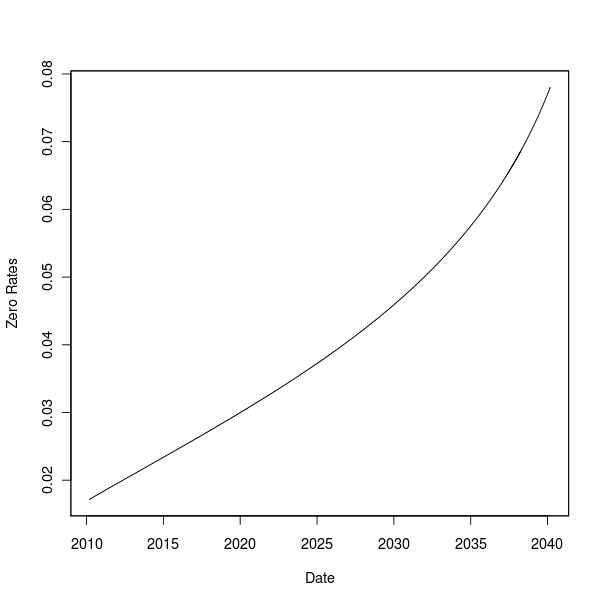
\includegraphics{figures/fittedBondCurve.png}}
\end{center}
\end{frame}



\begin{frame}
	\frametitle{Fixed Income in RQuantLib}
	\framesubtitle{Examples: Bond pricing}	
In this example, we construct a bond discounting term structure and a swap term structure then use them to price a zero coupon bond and a fixed rate bond. 
\vskip5pt
\pagecolor{bgcolor}
\noindent
\scriptsize
\ttfamily
\hlstd{fixingDays\ }\hlsym{$<${-}\ }\hlstd{}\hlnum{3}\hspace*{\fill}\\
\hlstd{settlementDays\ }\hlsym{$<${-}\ }\hlstd{}\hlnum{3}\hspace*{\fill}\\
\hlstd{settlementDate\ }\hlsym{$<${-}\ }\hlstd{}\hlkwc{as.Date}\hlstd{}\hlsym{(}\hlstd{}\hlstr{'2008{-}09{-}18'}\hlstd{}\hlsym{)}\hspace*{\fill}\\
\hlstd{todaysDate\ }\hlsym{$<${-}\ }\hlstd{settlementDate\ }\hlsym{{-}\ }\hlstd{fixingDays}\hspace*{\fill}\\
\hlslc{\#begin\ to\ set\ up\ bond\ discounting\ term\ structure}\hspace*{\fill}\\
\hlstd{lengths\ }\hlsym{$<${-}\ }\hlstd{}\hlkwc{c}\hlstd{}\hlsym{(}\hlstd{}\hlnum{5}\hlstd{}\hlsym{,\ }\hlstd{}\hlnum{6}\hlstd{}\hlsym{,\ }\hlstd{}\hlnum{7}\hlstd{}\hlsym{,\ }\hlstd{}\hlnum{16}\hlstd{}\hlsym{,\ }\hlstd{}\hlnum{48}\hlstd{}\hlsym{)}\hspace*{\fill}\\
\hlstd{coupons\ }\hlsym{$<${-}\ }\hlstd{}\hlkwc{c}\hlstd{}\hlsym{(}\hlstd{}\hlnum{0.02375}\hlstd{}\hlsym{,\ }\hlstd{}\hlnum{0.04625}\hlstd{}\hlsym{,\ }\hlstd{}\hlnum{0.03125}\hlstd{}\hlsym{,}\hspace*{\fill}\\
\hlstd{}\hlstd{\ \ \ \ \ \ \ \ \ \ \ \ \ }\hlstd{}\hlnum{0.04000}\hlstd{}\hlsym{,\ }\hlstd{}\hlnum{0.04500}\hlstd{}\hlsym{)}\hspace*{\fill}\\
\hlstd{marketQuotes\ }\hlsym{$<${-}\ }\hlstd{}\hlkwc{c}\hlstd{}\hlsym{(}\hlstd{}\hlnum{100.390625}\hlstd{}\hlsym{,\ }\hlstd{}\hlnum{106.21875}\hlstd{}\hlsym{,}\hspace*{\fill}\\
\hlstd{}\hlstd{\ \ \ \ \ \ \ \ \ \ \ \ \ \ \ \ \ \ }\hlstd{}\hlnum{100.59375}\hlstd{}\hlsym{,\ }\hlstd{}\hlnum{101.6875}\hlstd{}\hlsym{,\ }\hlstd{}\hlnum{102.140625}\hlstd{}\hlsym{)}\hspace*{\fill}\\
\hlstd{dateparams\ }\hlsym{$<${-}\ }\hlstd{}\hlkwc{list}\hlstd{}\hlsym{(}\hlstd{settlementDays}\hlsym{=}\hlstd{settlementDays}\hlsym{,}\hspace*{\fill}\\
\hlstd{}\hlstd{\ \ \ \ \ \ \ \ \ \ \ \ \ \ \ \ \ \ \ }\hlstd{period}\hlsym{=}\hlstd{}\hlnum{2}\hlstd{}\hlsym{,\ }\hlstd{dayCounter}\hlsym{=}\hlstd{}\hlstr{"ActualActual"}\hlstd{}\hlsym{,}\hspace*{\fill}\\
\hlstd{}\hlstd{\ \ \ \ \ \ \ \ \ \ \ \ \ \ \ \ \ \ \ }\hlstd{businessDayConvention\ }\hlsym{=}\hlstd{}\hlstr{"Unadjusted"}\hlstd{}\hlsym{)}\hspace*{\fill}\\
\hlstd{curveparams\ }\hlsym{$<${-}\ }\hlstd{}\hlkwc{list}\hlstd{}\hlsym{(}\hlstd{method}\hlsym{=}\hlstd{}\hlstr{"ExponentialSplinesFitting"}\hlstd{}\hlsym{,}\hspace*{\fill}\\
\hlstd{}\hlstd{\ \ \ \ \ \ \ \ \ \ \ \ \ \ \ \ \ \ \ \ }\hlstd{origDate}\hlsym{=}\hlstd{todaysDate}\hlsym{)}\hspace*{\fill}\\
\hlstd{bondDsctTsr\ }\hlsym{$<${-}\ }\hlstd{FittedBondCurve}\hlsym{(}\hlstd{curveparams}\hlsym{,\ }\hlstd{lengths}\hlsym{,}\hspace*{\fill}\\
\hlstd{}\hlstd{\ \ \ \ \ \ \ \ \ \ \ \ \ \ \ \ \ \ \ \ \ \ \ \ \ \ \ \ \ \ \ }\hlstd{coupons}\hlsym{,\ }\hlstd{marketQuotes}\hlsym{,}\hspace*{\fill}\\
\hlstd{}\hlstd{\ \ \ \ \ \ \ \ \ \ \ \ \ \ \ \ \ \ \ \ \ \ \ \ \ \ \ \ \ \ \ }\hlstd{dateparams}\hlsym{)}\hlstd{}\hspace*{\fill}\\
\mbox{}
\normalfont
\end{frame}

\begin{frame}
	\frametitle{Fixed Income in RQuantLib}
	\framesubtitle{Examples: Bond pricing}
\pagecolor{bgcolor}
\noindent
\scriptsize
\ttfamily
\hlstd{}\hlslc{\#begin\ to\ set\ up\ swap\ term\ structure}\hspace*{\fill}\\
\hlstd{swp.tsr.params\ }\hlsym{$<${-}\ }\hlstd{}\hlkwc{list}\hlstd{}\hlsym{(}\hlstd{tradeDate}\hlsym{=}\hlstd{todaysDate}\hlsym{,}\hspace*{\fill}\\
\hlstd{}\hlstd{\ \ \ \ \ \ \ \ \ \ \ \ \ \ \ \ \ \ \ \ \ \ \ }\hlstd{settleDate}\hlsym{=}\hlstd{todaysDate}\hlsym{+}\hlstd{}\hlnum{2}\hlstd{}\hlsym{,}\hspace*{\fill}\\
\hlstd{}\hlstd{\ \ \ \ \ \ \ \ \ \ \ \ \ \ \ \ \ \ \ \ \ \ \ }\hlstd{}\hlkwc{dt}\hlstd{}\hlsym{=}\hlstd{}\hlnum{0.25}\hlstd{}\hlsym{,}\hspace*{\fill}\\
\hlstd{}\hlstd{\ \ \ \ \ \ \ \ \ \ \ \ \ \ \ \ \ \ \ \ \ \ \ }\hlstd{interpWhat}\hlsym{=}\hlstd{}\hlstr{"discount"}\hlstd{}\hlsym{,}\hspace*{\fill}\\
\hlstd{}\hlstd{\ \ \ \ \ \ \ \ \ \ \ \ \ \ \ \ \ \ \ \ \ \ \ }\hlstd{interpHow}\hlsym{=}\hlstd{}\hlstr{"loglinear"}\hlstd{}\hlsym{)}\hspace*{\fill}\\
\hlstd{market.quotes\ }\hlsym{$<${-}\ }\hlstd{}\hlkwc{list}\hlstd{}\hlsym{(}\hlstd{d1w}\hlsym{=}\hlstd{}\hlnum{0.043375}\hlstd{}\hlsym{,\ }\hlstd{d1m}\hlsym{=}\hlstd{}\hlnum{0.031875}\hlstd{}\hlsym{,}\hspace*{\fill}\\
\hlstd{}\hlstd{\ \ \ \ \ \ \ \ \ \ \ \ \ \ \ \ \ \ \ \ \ \ }\hlstd{d3m}\hlsym{=}\hlstd{}\hlnum{0.0320375}\hlstd{}\hlsym{,\ }\hlstd{d6m}\hlsym{=}\hlstd{}\hlnum{0.03385}\hlstd{}\hlsym{,}\hspace*{\fill}\\
\hlstd{}\hlstd{\ \ \ \ \ \ \ \ \ \ \ \ \ \ \ \ \ \ \ \ \ \ }\hlstd{d9m}\hlsym{=}\hlstd{}\hlnum{0.0338125}\hlstd{}\hlsym{,\ }\hlstd{d1y}\hlsym{=}\hlstd{}\hlnum{0.0335125}\hlstd{}\hlsym{,}\hspace*{\fill}\\
\hlstd{}\hlstd{\ \ \ \ \ \ \ \ \ \ \ \ \ \ \ \ \ \ \ \ \ \ }\hlstd{s2y}\hlsym{=}\hlstd{}\hlnum{0.0295}\hlstd{}\hlsym{,\ }\hlstd{s3y}\hlsym{=}\hlstd{}\hlnum{0.0323}\hlstd{}\hlsym{,}\hspace*{\fill}\\
\hlstd{}\hlstd{\ \ \ \ \ \ \ \ \ \ \ \ \ \ \ \ \ \ \ \ \ \ }\hlstd{s5y}\hlsym{=}\hlstd{}\hlnum{0.0359}\hlstd{}\hlsym{,\ }\hlstd{s10y}\hlsym{=}\hlstd{}\hlnum{0.0412}\hlstd{}\hlsym{,}\hspace*{\fill}\\
\hlstd{}\hlstd{\ \ \ \ \ \ \ \ \ \ \ \ \ \ \ \ \ \ \ \ \ \ }\hlstd{s15y}\hlsym{=}\hlstd{}\hlnum{0.0433}\hlstd{}\hlsym{)}\hspace*{\fill}\\
\hlstd{depoSwpTsr\ }\hlsym{$<${-}\ }\hlstd{DiscountCurve}\hlsym{(}\hlstd{swp.tsr.params}\hlsym{,\ }\hlstd{market.quotes}\hlsym{)}\hlstd{}\hspace*{\fill}\\
\mbox{}
\normalfont
\end{frame}


\begin{frame}[fragile]
	\frametitle{Fixed Income in RQuantLib}
	\framesubtitle{Examples: Bond pricing}	
\pagecolor{bgcolor}
\noindent
\scriptsize
\ttfamily
\hlstd{}\hlslc{\#Zero{-}Coupon\ Bond}\hspace*{\fill}\\
\hlstd{zc.bond.param\ }\hlsym{$<${-}\ }\hlstd{}\hlkwc{list}\hlstd{}\hlsym{(}\hspace*{\fill}\\
\hlstd{}\hlstd{\ \ \ \ \ \ \ \ \ \ \ \ \ \ }\hlstd{maturityDate}\hlsym{=}\hlstd{}\hlkwc{as.Date}\hlstd{}\hlsym{(}\hlstd{}\hlstr{'2013{-}08{-}15'}\hlstd{}\hlsym{),}\hspace*{\fill}\\
\hlstd{}\hlstd{\ \ \ \ \ \ \ \ \ \ \ \ \ \ }\hlstd{issueDate}\hlsym{=}\hlstd{}\hlkwc{as.Date}\hlstd{}\hlsym{(}\hlstd{}\hlstr{'2003{-}08{-}15'}\hlstd{}\hlsym{),}\hspace*{\fill}\\
\hlstd{}\hlstd{\ \ \ \ \ \ \ \ \ \ \ \ \ \ }\hlstd{redemption}\hlsym{=}\hlstd{}\hlnum{116.92}\hlstd{}\hlsym{)}\hspace*{\fill}\\
\hlstd{zc.bond.dateparam\ }\hlsym{$<${-}\ }\hlstd{}\hlkwc{list}\hlstd{}\hlsym{(}\hspace*{\fill}\\
\hlstd{}\hlstd{\ \ \ \ \ \ \ \ \ \ \ \ \ \ }\hlstd{refDate}\hlsym{=}\hlstd{todaysDate}\hlsym{,}\hspace*{\fill}\\
\hlstd{}\hlstd{\ \ \ \ \ \ \ \ \ \ \ \ \ \ }\hlstd{settlementDays}\hlsym{=}\hlstd{settlementDays}\hlsym{,}\hspace*{\fill}\\
\hlstd{}\hlstd{\ \ \ \ \ \ \ \ \ \ \ \ \ \ }\hlstd{businessDayConvention}\hlsym{=}\hlstd{}\hlstr{'Following'}\hlstd{}\hlsym{)}\hspace*{\fill}\\
\hlstd{ZeroCouponBond}\hlsym{(}\hlstd{zc.bond.param}\hlsym{,}\hspace*{\fill}\\
\hlstd{}\hlstd{\ \ \ \ \ \ \ \ \ \ \ \ \ \ \ }\hlstd{bondDsctTsr}\hlsym{,}\hspace*{\fill}\\
\hlstd{}\hlstd{\ \ \ \ \ \ \ \ \ \ \ \ \ \ \ }\hlstd{zc.bond.dateparam}\hlsym{)}\hlstd{}\hspace*{\fill}\\
\mbox{}
\normalfont
\end{frame}

\begin{frame}[fragile]
	\frametitle{Fixed Income in RQuantLib}
	\framesubtitle{Examples: Bond pricing}
\pagecolor{bgcolor}
\noindent
\scriptsize
\ttfamily
\hlstd{}\hlslc{\#Fixed{-}Coupon\ Bond}\hspace*{\fill}\\
\hlstd{fixed.bond.param\ }\hlsym{$<${-}\ }\hlstd{}\hlkwc{list}\hlstd{}\hlsym{(}\hspace*{\fill}\\
\hlstd{}\hlstd{\ \ \ \ \ \ \ \ \ \ \ \ \ \ \ \ \ }\hlstd{maturityDate}\hlsym{=}\hlstd{}\hlkwc{as.Date}\hlstd{}\hlsym{(}\hlstd{}\hlstr{'2017{-}05{-}15'}\hlstd{}\hlsym{),}\hspace*{\fill}\\
\hlstd{}\hlstd{\ \ \ \ \ \ \ \ \ \ \ \ \ \ \ \ \ }\hlstd{issueDate}\hlsym{=}\hlstd{}\hlkwc{as.Date}\hlstd{}\hlsym{(}\hlstd{}\hlstr{'2007{-}05{-}15'}\hlstd{}\hlsym{),}\hspace*{\fill}\\
\hlstd{}\hlstd{\ \ \ \ \ \ \ \ \ \ \ \ \ \ \ \ \ }\hlstd{redemption}\hlsym{=}\hlstd{}\hlnum{100}\hlstd{}\hlsym{,}\hspace*{\fill}\\
\hlstd{}\hlstd{\ \ \ \ \ \ \ \ \ \ \ \ \ \ \ \ \ }\hlstd{effectiveDate}\hlsym{=}\hlstd{}\hlkwc{as.Date}\hlstd{}\hlsym{(}\hlstd{}\hlstr{'2007{-}05{-}15'}\hlstd{}\hlsym{))}\hspace*{\fill}\\
\hlstd{fixed.bond.dateparam\ }\hlsym{$<${-}\ }\hlstd{}\hlkwc{list}\hlstd{}\hlsym{(}\hspace*{\fill}\\
\hlstd{}\hlstd{\ \ \ \ \ \ \ \ \ \ \ \ \ \ \ \ \ }\hlstd{settlementDays}\hlsym{=}\hlstd{settlementDays}\hlsym{,}\hspace*{\fill}\\
\hlstd{}\hlstd{\ \ \ \ \ \ \ \ \ \ \ \ \ \ \ \ \ }\hlstd{dayCounter}\hlsym{=}\hlstd{}\hlstr{'ActualActual'}\hlstd{}\hlsym{,}\hspace*{\fill}\\
\hlstd{}\hlstd{\ \ \ \ \ \ \ \ \ \ \ \ \ \ \ \ \ }\hlstd{period}\hlsym{=}\hlstd{}\hlstr{'Semiannual'}\hlstd{}\hlsym{,}\hspace*{\fill}\\
\hlstd{}\hlstd{\ \ \ \ \ \ \ \ \ \ \ \ \ \ \ \ \ }\hlstd{businessDayConvention}\hlsym{=}\hlstd{}\hlstr{'Unadjusted'}\hlstd{}\hlsym{,}\hspace*{\fill}\\
\hlstd{}\hlstd{\ \ \ \ \ \ \ \ \ \ \ \ \ \ \ \ \ }\hlstd{terminationDateConvention}\hlsym{=}\hlstd{}\hlstr{'Unadjusted'}\hlstd{}\hlsym{,}\hspace*{\fill}\\
\hlstd{}\hlstd{\ \ \ \ \ \ \ \ \ \ \ \ \ \ \ \ \ }\hlstd{dateGeneration}\hlsym{=}\hlstd{}\hlstr{'Backward'}\hlstd{}\hlsym{,}\hspace*{\fill}\\
\hlstd{}\hlstd{\ \ \ \ \ \ \ \ \ \ \ \ \ \ \ \ \ }\hlstd{endOfMonth}\hlsym{=}\hlstd{}\hlnum{0}\hlstd{}\hlsym{)}\hspace*{\fill}\\
\hlstd{fixed.bond.coupon\ }\hlsym{$<${-}\ }\hlstd{}\hlkwc{c}\hlstd{}\hlsym{(}\hlstd{}\hlnum{0.045}\hlstd{}\hlsym{)}\hspace*{\fill}\\
\hlstd{FixedRateBond}\hlsym{(}\hlstd{fixed.bond.param}\hlsym{,\ }\hlstd{fixed.bond.coupon}\hlsym{,}\hspace*{\fill}\\
\hlstd{}\hlstd{\ \ \ \ \ \ \ \ \ \ \ \ \ \ }\hlstd{bondDsctTsr}\hlsym{,\ }\hlstd{fixed.bond.dateparam}\hlsym{)}\hlstd{}\hspace*{\fill}\\
\mbox{}
\normalfont
\end{frame}

\begin{frame}[fragile]
	\frametitle{Fixed Income in RQuantLib}
	\framesubtitle{Examples: Convertible Bond from Matlab's Fixed Income Toolbox}	
	\scriptsize
Perform a spread effect analysis of a 4\%-coupon convertible bond callable at 110 at the end of the second year, maturing at par in 5 years, with yield to maturity of 5\% and spread (of YTM versus 5-year treasury) of 0, 50, 100, and 150 basis points. The underlying stock pays no dividend. 
\lstset{language=Matlab,basicstyle=\tiny}
	\begin{lstlisting}
RiskFreeRate = 0.05;	Sigma        = 0.3;
ConvRatio    = 1;   	NumSteps     = 200;
IssueDate    = datenum('2-Jan-2002');
Settle       = datenum('2-Jan-2002');
Maturity     = datenum('2-Jan-2007');
CouponRate   = 0.04;    Period       = 2; Basis        = 1;		EndMonthRule = 1;
DividendType = 0;		DividendInfo = [];
CallInfo     = [datenum('2-Jan-2004'), 110]; 
CallType     = 1;		TreeType     = 1;   
% Nested loop accross prices and static spread dimensions to compute convertible prices.
for j = 0:0.005:0.015;
StaticSpread = j;
      for i = 0:10:100
          Price = 40+i;
          [CbMatrix, UndMatrix, DebtMatrix, EqtyMatrix] =  cbprice(RiskFreeRate, StaticSpread, Sigma, Price, ConvRatio, NumSteps, IssueDate, Settle, Maturity, CouponRate, Period, Basis, EndMonthRule, DividendType, DividendInfo, CallType, CallInfo, TreeType);   
           convprice(i/10+1,j*200+1) =  CbMatrix(1,1);
           stock(i/10+1,j*200+1)     =  Price;
        end    
end
\end{lstlisting}
\end{frame}

\begin{frame}[fragile]
 \begin{columns}
 \column{1.5in}
\lstset{language=Matlab,basicstyle=\tiny}
	\begin{lstlisting}
   plot(stock, convprice);
    legend({'+0 bp'; '+50 bp'; '+100 bp'; '+150 bp'});
    title ('Effect of Spread using Trinomial tree - 200 steps')
    xlabel('Stock Price');
    ylabel('Convertible Price');
    text(50, 150, ['Coupon 4% semiannual.', sprintf('\n'), ...
         '110 Call-on-clean after two years.' sprintf('\n'), ...
         'Maturing at par in five years.'],'fontweight','Bold')
 	\end{lstlisting}
 	
  \column{2.8in}
\begin{center}
\resizebox{75mm}{!}{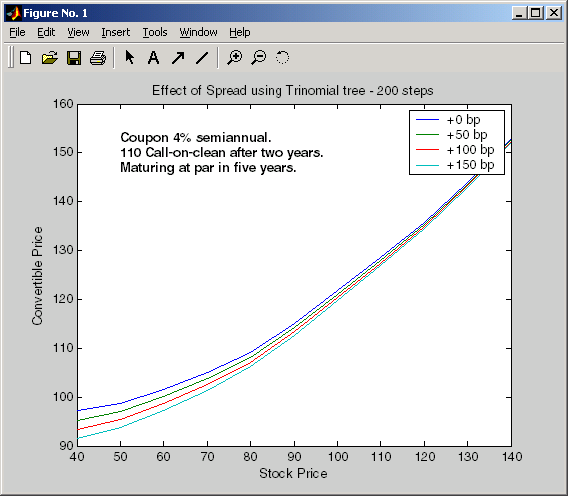
\includegraphics{figures/cbspread.png}}
\end{center}

\end{columns}
\end{frame}

\begin{frame}
Doing it in R using RQuantLib....
\vskip5pt
\tiny
\pagecolor{bgcolor}
\noindent
\ttfamily
\hlstd{params\ }\hlsym{$<${-}\ }\hlstd{}\hlkwc{list}\hlstd{}\hlsym{(}\hlstd{tradeDate}\hlsym{=}\hlstd{}\hlkwc{as.Date}\hlstd{}\hlsym{(}\hlstd{}\hlstr{'2002{-}01{-}02'}\hlstd{}\hlsym{),}\hspace*{\fill}\\
\hlstd{}\hlstd{\ \ \ \ \ \ \ \ \ \ \ \ \ \ \ }\hlstd{settleDate}\hlsym{=}\hlstd{}\hlkwc{as.Date}\hlstd{}\hlsym{(}\hlstd{}\hlstr{'2002{-}01{-}02'}\hlstd{}\hlsym{),}\hspace*{\fill}\\
\hlstd{}\hlstd{\ \ \ \ \ \ \ \ \ \ \ \ \ \ \ }\hlstd{}\hlkwc{dt}\hlstd{}\hlsym{=}\hlstd{}\hlnum{.25}\hlstd{}\hlsym{,}\hspace*{\fill}\\
\hlstd{}\hlstd{\ \ \ \ \ \ \ \ \ \ \ \ \ \ \ }\hlstd{interpWhat}\hlsym{=}\hlstd{}\hlstr{"discount"}\hlstd{}\hlsym{,}\hspace*{\fill}\\
\hlstd{}\hlstd{\ \ \ \ \ \ \ \ \ \ \ \ \ \ \ }\hlstd{interpHow}\hlsym{=}\hlstd{}\hlstr{"loglinear"}\hlstd{}\hlsym{)}\hspace*{\fill}\\
\hlstd{times\ }\hlsym{$<${-}\ }\hlstd{}\hlkwc{seq}\hlstd{}\hlsym{(}\hlstd{}\hlnum{0}\hlstd{}\hlsym{,}\hlstd{}\hlnum{10}\hlstd{}\hlsym{,}\hlstd{}\hlnum{.1}\hlstd{}\hlsym{)}\hspace*{\fill}\\
\hlstd{\hspace*{\fill}\\
RiskFreeRate\ }\hlsym{$<${-}\ }\hlstd{DiscountCurve}\hlsym{(}\hlstd{params}\hlsym{,\ }\hlstd{}\hlkwc{list}\hlstd{}\hlsym{(}\hlstd{flat}\hlsym{=}\hlstd{}\hlnum{0.05}\hlstd{}\hlsym{),}\hlstd{times}\hlsym{)}\hspace*{\fill}\\
\hlstd{Sigma\ }\hlsym{$<${-}\ }\hlstd{}\hlnum{0.3}\hspace*{\fill}\\
\hlstd{ConvRatio\ }\hlsym{$<${-}\ }\hlstd{}\hlnum{1}\hspace*{\fill}\\
\hlstd{issueDate\ }\hlsym{$<${-}\ }\hlstd{}\hlkwc{as.Date}\hlstd{}\hlsym{(}\hlstd{}\hlstr{'2002{-}01{-}02'}\hlstd{}\hlsym{)}\hspace*{\fill}\\
\hlstd{settleDate\ }\hlsym{$<${-}\ }\hlstd{}\hlkwc{as.Date}\hlstd{}\hlsym{(}\hlstd{}\hlstr{'2002{-}01{-}02'}\hlstd{}\hlsym{)}\hspace*{\fill}\\
\hlstd{maturityDate\ }\hlsym{$<${-}\ }\hlstd{}\hlkwc{as.Date}\hlstd{}\hlsym{(}\hlstd{}\hlstr{'2007{-}01{-}02'}\hlstd{}\hlsym{)}\hspace*{\fill}\\
\hlstd{dividendYield\ }\hlsym{$<${-}\ }\hlstd{DiscountCurve}\hlsym{(}\hlstd{params}\hlsym{,\ }\hlstd{}\hlkwc{list}\hlstd{}\hlsym{(}\hlstd{flat}\hlsym{=}\hlstd{}\hlnum{0.01}\hlstd{}\hlsym{),}\hlstd{times}\hlsym{)}\hspace*{\fill}\\
\hlstd{dividendSchedule\ }\hlsym{$<${-}\ }\hlstd{}\hlkwc{data.frame}\hlstd{}\hlsym{(}\hlstd{Type}\hlsym{=}\hlstd{}\hlkwc{character}\hlstd{}\hlsym{(}\hlstd{}\hlnum{0}\hlstd{}\hlsym{),}\hspace*{\fill}\\
\hlstd{}\hlstd{\ \ \ \ \ \ \ \ \ \ \ \ \ \ \ \ \ \ \ \ \ \ \ \ \ \ \ \ \ \ \ }\hlstd{Amount}\hlsym{=}\hlstd{}\hlkwc{numeric}\hlstd{}\hlsym{(}\hlstd{}\hlnum{0}\hlstd{}\hlsym{),}\hspace*{\fill}\\
\hlstd{}\hlstd{\ \ \ \ \ \ \ \ \ \ \ \ \ \ \ \ \ \ \ \ \ \ \ \ \ \ \ \ \ \ \ }\hlstd{Rate}\hlsym{=}\hlstd{}\hlkwc{numeric}\hlstd{}\hlsym{(}\hlstd{}\hlnum{0}\hlstd{}\hlsym{),}\hspace*{\fill}\\
\hlstd{}\hlstd{\ \ \ \ \ \ \ \ \ \ \ \ \ \ \ \ \ \ \ \ \ \ \ \ \ \ \ \ \ \ \ }\hlstd{Date}\hlsym{=}\hlstd{}\hlkwc{as.Date}\hlstd{}\hlsym{(}\hlstd{}\hlkwc{character}\hlstd{}\hlsym{(}\hlstd{}\hlnum{0}\hlstd{}\hlsym{)))}\hspace*{\fill}\\
\hlstd{callabilitySchedule\ }\hlsym{$<${-}\ }\hlstd{}\hlkwc{data.frame}\hlstd{}\hlsym{(}\hlstd{Price}\hlsym{=}\hlstd{}\hlnum{110}\hlstd{}\hlsym{,\ }\hlstd{Type}\hlsym{=}\hlstd{}\hlnum{0}\hlstd{}\hlsym{,}\hspace*{\fill}\\
\hlstd{}\hlstd{\ \ \ \ \ \ \ \ \ \ \ \ \ \ \ \ \ \ \ \ \ \ \ \ \ \ \ \ \ \ \ \ \ \ }\hlstd{Date}\hlsym{=}\hlstd{}\hlkwc{as.Date}\hlstd{}\hlsym{(}\hlstd{}\hlstr{'2004{-}01{-}02'}\hlstd{}\hlsym{))}\hspace*{\fill}\\
\hlstd{process\ }\hlsym{$<${-}\ }\hlstd{}\hlkwc{list}\hlstd{}\hlsym{(}\hlstd{underlying}\hlsym{=}\hlstd{}\hlnum{40}\hlstd{}\hlsym{,\ }\hlstd{divYield}\hlsym{=}\hlstd{dividendYield}\hlsym{,}\hspace*{\fill}\\
\hlstd{}\hlstd{\ \ \ \ \ \ \ \ \ \ \ \ \ \ \ \ }\hlstd{rff}\hlsym{=}\hlstd{RiskFreeRate}\hlsym{,\ }\hlstd{volatility}\hlsym{=}\hlstd{Sigma}\hlsym{)}\hspace*{\fill}\\
\hlstd{\hspace*{\fill}\\
bondparams\ }\hlsym{$<${-}\ }\hlstd{}\hlkwc{list}\hlstd{}\hlsym{(}\hlstd{exercise}\hlsym{=}\hlstd{}\hlstr{"eu"}\hlstd{}\hlsym{,\ }\hlstd{faceAmount}\hlsym{=}\hlstd{}\hlnum{100}\hlstd{}\hlsym{,}\hspace*{\fill}\\
\hlstd{}\hlstd{\ \ \ \ \ \ \ \ \ \ \ \ \ \ \ \ \ \ \ }\hlstd{divSch}\hlsym{=}\hlstd{dividendSchedule}\hlsym{,}\hspace*{\fill}\\
\hlstd{}\hlstd{\ \ \ \ \ \ \ \ \ \ \ \ \ \ \ \ \ \ \ }\hlstd{callSch}\hlsym{=}\hlstd{callabilitySchedule}\hlsym{,}\hspace*{\fill}\\
\hlstd{}\hlstd{\ \ \ \ \ \ \ \ \ \ \ \ \ \ \ \ \ \ \ }\hlstd{redemption}\hlsym{=}\hlstd{}\hlnum{100}\hlstd{}\hlsym{,}\hspace*{\fill}\\
\hlstd{}\hlstd{\ \ \ \ \ \ \ \ \ \ \ \ \ \ \ \ \ \ \ }\hlstd{creditSpread}\hlsym{=}\hlstd{}\hlnum{0.005}\hlstd{}\hlsym{,}\hspace*{\fill}\\
\hlstd{}\hlstd{\ \ \ \ \ \ \ \ \ \ \ \ \ \ \ \ \ \ \ }\hlstd{conversionRatio}\hlsym{=}\hlstd{ConvRatio}\hlsym{,}\hspace*{\fill}\\
\hlstd{}\hlstd{\ \ \ \ \ \ \ \ \ \ \ \ \ \ \ \ \ \ \ }\hlstd{issueDate}\hlsym{=}\hlstd{issueDate}\hlsym{,}\hspace*{\fill}\\
\hlstd{}\hlstd{\ \ \ \ \ \ \ \ \ \ \ \ \ \ \ \ \ \ \ }\hlstd{maturityDate}\hlsym{=}\hlstd{maturityDate}\hlsym{)}\hlstd{}\hspace*{\fill}\\
\mbox{}
\normalfont
\end{frame}

\begin{frame}
\scriptsize
\pagecolor{bgcolor}
\noindent
\tiny
\ttfamily
\hlstd{\hspace*{\fill}\\
dateparams\ }\hlsym{$<${-}\ }\hlstd{}\hlkwc{list}\hlstd{}\hlsym{(}\hlstd{settlementDays}\hlsym{=}\hlstd{}\hlnum{3}\hlstd{}\hlsym{,}\hspace*{\fill}\\
\hlstd{}\hlstd{\ \ \ \ \ \ \ \ \ \ \ \ \ \ \ \ \ \ \ }\hlstd{dayCounter}\hlsym{=}\hlstd{}\hlstr{"Thirty360"}\hlstd{}\hlsym{,}\hspace*{\fill}\\
\hlstd{}\hlstd{\ \ \ \ \ \ \ \ \ \ \ \ \ \ \ \ \ \ \ }\hlstd{period}\hlsym{=}\hlstd{}\hlstr{"Semiannual"}\hlstd{}\hlsym{,\ }\hlstd{calendar}\hlsym{=}\hlstd{}\hlstr{"us"}\hlstd{}\hlsym{,}\hspace*{\fill}\\
\hlstd{}\hlstd{\ \ \ \ \ \ \ \ \ \ \ \ \ \ \ \ \ \ \ }\hlstd{businessDayConvention}\hlsym{=}\hlstd{}\hlstr{"Following"}\hlstd{}\hlsym{,}\hspace*{\fill}\\
\hlstd{}\hlstd{\ \ \ \ \ \ \ \ \ \ \ \ \ \ \ \ \ \ \ }\hlstd{todayDate}\hlsym{=}\hlstd{issueDate}\hlsym{)}\hspace*{\fill}\\
\hlstd{coupon\ }\hlsym{$<${-}\ }\hlstd{}\hlnum{0.04}\hspace*{\fill}\\
\hlstd{\hspace*{\fill}\\
ret\ }\hlsym{$<${-}\ }\hlstd{}\hlkwc{data.frame}\hlstd{}\hlsym{()}\hspace*{\fill}\\
\hlstd{}\hlkwa{for\ }\hlstd{}\hlsym{(}\hlstd{s\ }\hlkwa{in\ }\hlstd{}\hlkwc{c}\hlstd{}\hlsym{(}\hlstd{}\hlnum{0}\hlstd{}\hlsym{,\ }\hlstd{}\hlnum{0.005}\hlstd{}\hlsym{,\ }\hlstd{}\hlnum{0.010}\hlstd{}\hlsym{,\ }\hlstd{}\hlnum{0.015}\hlstd{}\hlsym{))\{}\hspace*{\fill}\\
\hlstd{\hspace*{\fill}\\
}\hlstd{\ \ }\hlstd{x\ }\hlsym{$<${-}\ }\hlstd{}\hlkwc{c}\hlstd{}\hlsym{()}\hspace*{\fill}\\
\hlstd{}\hlstd{\ \ }\hlstd{y\ }\hlsym{$<${-}\ }\hlstd{}\hlkwc{c}\hlstd{}\hlsym{()}\hspace*{\fill}\\
\hlstd{}\hlstd{\ \ }\hlstd{i\ }\hlsym{$<${-}\ }\hlstd{}\hlnum{1}\hspace*{\fill}\\
\hlstd{}\hlstd{\ \ }\hlstd{}\hlkwa{for\ }\hlstd{}\hlsym{(}\hlstd{p\ }\hlkwa{in\ }\hlstd{}\hlkwc{seq}\hlstd{}\hlsym{(}\hlstd{}\hlnum{0}\hlstd{}\hlsym{,\ }\hlstd{}\hlnum{100}\hlstd{}\hlsym{,\ }\hlstd{}\hlkwc{by\ }\hlstd{}\hlsym{=\ }\hlstd{}\hlnum{10}\hlstd{}\hlsym{))\ \{}\hspace*{\fill}\\
\hlstd{}\hlstd{\ \ \ \ }\hlstd{process\$underlying\ }\hlsym{$<${-}\ }\hlstd{}\hlnum{40}\hlstd{}\hlsym{+}\hlstd{p\hspace*{\fill}\\
}\hlstd{\ \ \ \ }\hlstd{bondparams\$creditSpread\ }\hlsym{$<${-}\ }\hlstd{s\hspace*{\fill}\\
}\hlstd{\ \ \ \ }\hlstd{}\hlkwc{t\ }\hlstd{}\hlsym{$<${-}\ }\hlstd{ConvertibleFixedCouponBond}\hlsym{(}\hlstd{bondparams}\hlsym{,}\hspace*{\fill}\\
\hlstd{}\hlstd{\ \ \ \ \ \ \ \ \ \ \ \ \ \ \ \ \ \ \ \ \ \ \ \ \ \ \ \ \ \ \ \ \ \ \ \ }\hlstd{coupon}\hlsym{,}\hspace*{\fill}\\
\hlstd{}\hlstd{\ \ \ \ \ \ \ \ \ \ \ \ \ \ \ \ \ \ \ \ \ \ \ \ \ \ \ \ \ \ \ \ \ \ \ \ }\hlstd{process}\hlsym{,}\hspace*{\fill}\\
\hlstd{}\hlstd{\ \ \ \ \ \ \ \ \ \ \ \ \ \ \ \ \ \ \ \ \ \ \ \ \ \ \ \ \ \ \ \ \ \ \ \ }\hlstd{dateparams}\hlsym{)}\hspace*{\fill}\\
\hlstd{}\hlstd{\ \ \ \ }\hlstd{x}\hlsym{{[}}\hlstd{i}\hlsym{{]}\ $<${-}\ }\hlstd{p\ }\hlsym{+\ }\hlstd{}\hlnum{40}\hspace*{\fill}\\
\hlstd{}\hlstd{\ \ \ \ }\hlstd{y}\hlsym{{[}}\hlstd{i}\hlsym{{]}\ $<${-}\ }\hlstd{}\hlkwc{t}\hlstd{\$cleanPrice\hspace*{\fill}\\
}\hlstd{\ \ \ \ }\hlstd{i\ }\hlsym{$<${-}\ }\hlstd{i\ }\hlsym{+\ }\hlstd{}\hlnum{1}\hspace*{\fill}\\
\hlstd{}\hlstd{\ \ }\hlstd{}\hlsym{\}}\hspace*{\fill}\\
\hlstd{}\hlstd{\ \ }\hlstd{z\ }\hlsym{$<${-}\ }\hlstd{}\hlkwc{rep}\hlstd{}\hlsym{(}\hlstd{s}\hlsym{,\ }\hlstd{}\hlnum{11}\hlstd{}\hlsym{)}\hspace*{\fill}\\
\hlstd{}\hlstd{\ \ }\hlstd{ret\ }\hlsym{$<${-}\ }\hlstd{}\hlkwc{rbind}\hlstd{}\hlsym{(}\hlstd{ret}\hlsym{,\ }\hlstd{}\hlkwc{data.frame}\hlstd{}\hlsym{(}\hlstd{Stock}\hlsym{=}\hlstd{x}\hlsym{,}\hlstd{ConvPrice}\hlsym{=}\hlstd{y}\hlsym{,}\hlstd{z}\hlsym{))}\hspace*{\fill}\\
\hlstd{}\hlsym{\}}\hspace*{\fill}\\

\hlstd{}\hspace*{\fill}\\
\hspace*{\fill}\\
\hspace*{\fill}\\
\mbox{}
\normalfont
\end{frame}

\begin{frame}
\vskip10pt
\scriptsize
\pagecolor{bgcolor}
\noindent
\ttfamily
\hlstd{}\hlkwc{>library}\hlstd{}\hlsym{(}\hlstd{ggplot2}\hlsym{)}\hspace*{\fill}\\
\hlstd{>p\ }\hlsym{$<${-}\ }\hlstd{ggplot}\hlsym{(}\hlstd{ret}\hlsym{,\ }\hlstd{aes}\hlsym{(}\hlstd{Stock}\hlsym{,}\hlstd{ConvPrice}\hlsym{,\ }\hlstd{colour}\hlsym{=}\hlstd{}\hlkwc{factor}\hlstd{}\hlsym{(}\hlstd{z}\hlsym{)))}\hspace*{\fill}\\
\hlstd{>p\ }\hlsym{+\ }\hlstd{geom\textunderscore line}\hlsym{()\ +\ }\hlstd{scale\textunderscore colour\textunderscore discrete}\hlsym{(}\hlstd{}\hlstr{"Spread"}\hlstd{}\hlsym{)}\hspace*{\fill}\\
\hlstd{}\hlsym{+\ }\hlstd{opts}\hlsym{(}\hlstd{}\hlkwc{title}\hlstd{}\hlsym{=}\hlstd{}\hlstr{'Effect\ of\ spread\ on\ a\ convertible\ bond'}
\normalfont
\begin{center}
\resizebox{60mm}{!}{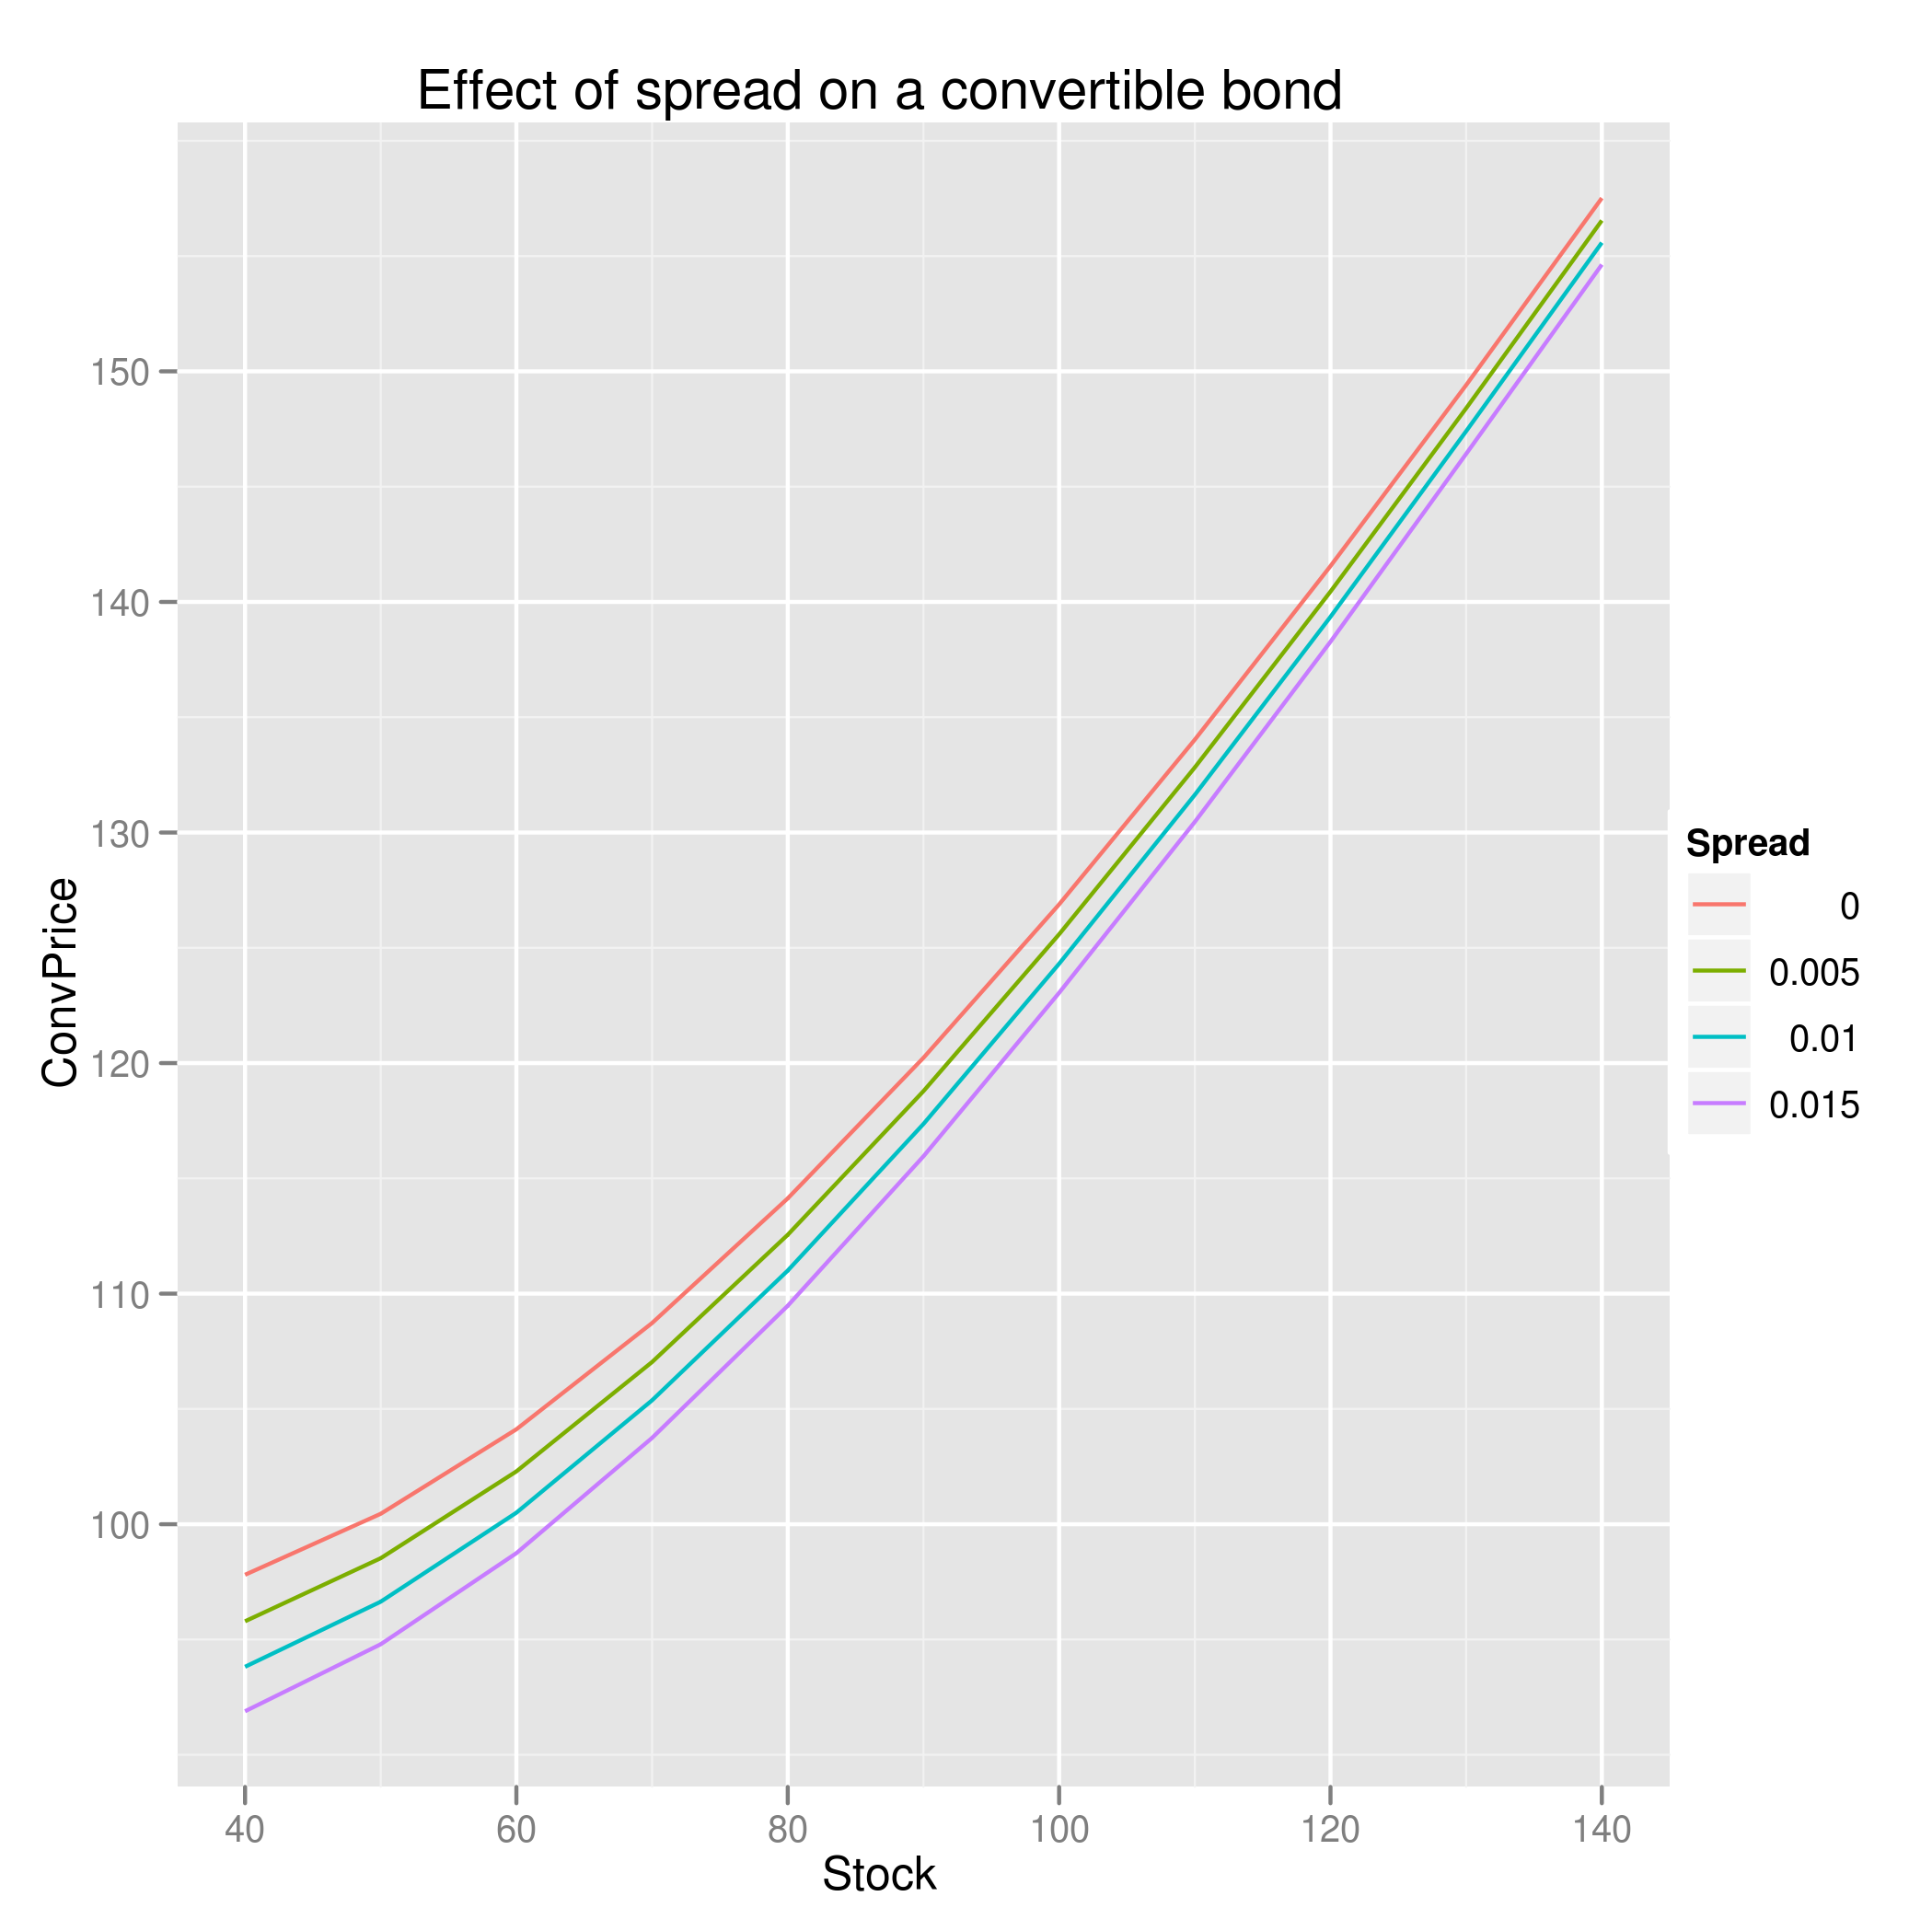
\includegraphics{figures/matlab_cbond.png}}
\end{center}
\end{frame}

\begin{frame}
	\frametitle{Fixed Income in RQuantLib}
	\framesubtitle{Graphical User Interface}		
RQuantLib also comes with an user interface via the 'traitr' package by professor John Verzani.
\begin{center}
	\resizebox{90mm}{!}{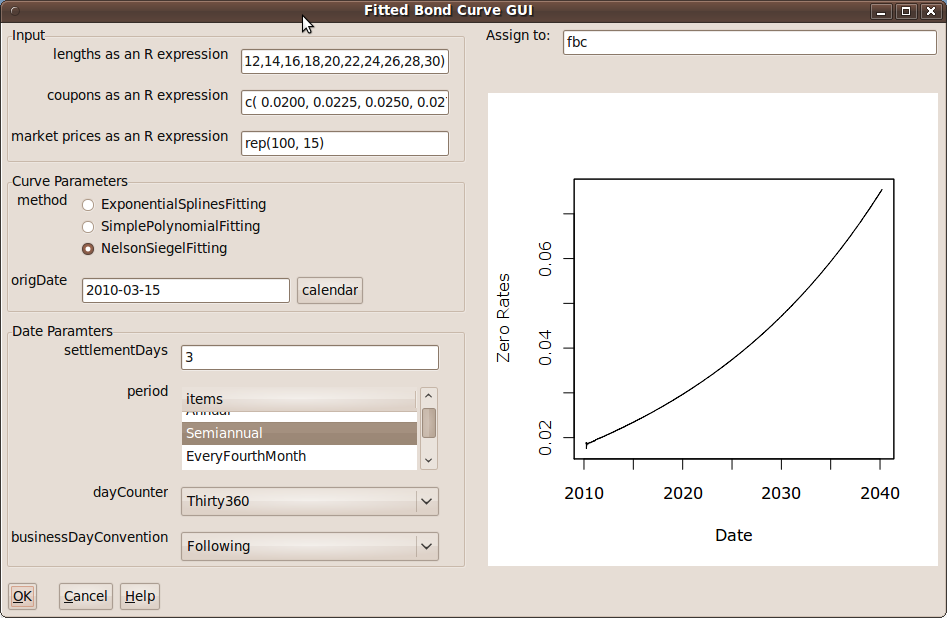
\includegraphics{figures/fbGUI.png}}
\end{center}
\end{frame}

\begin{frame}
	\frametitle{Fixed Income in RQuantLib}
	\framesubtitle{Graphical User Interface}	
\begin{center}
	\resizebox{110mm}{!}{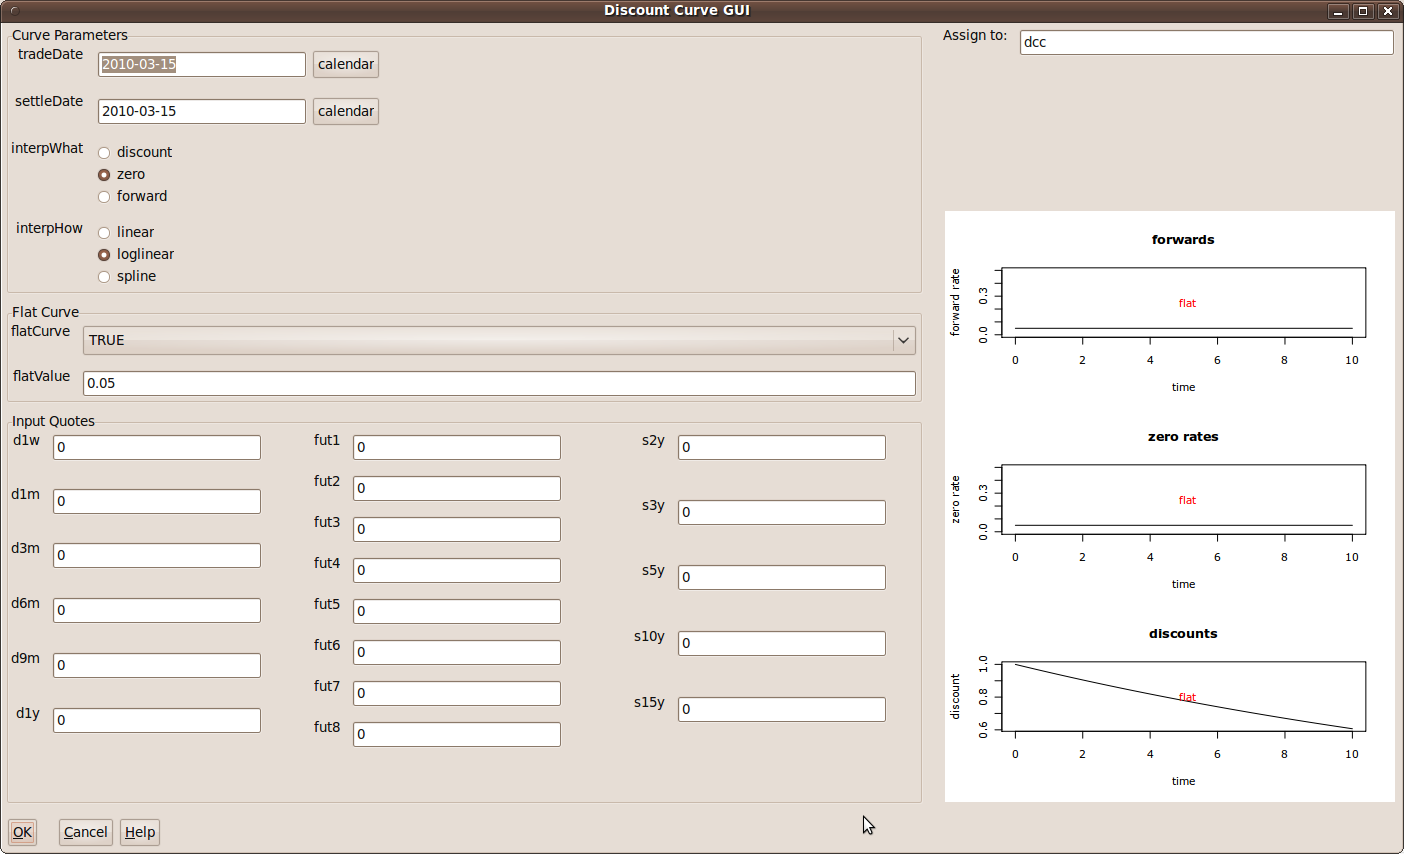
\includegraphics{figures/dcGUI.png}}
\end{center}
\end{frame}


\begin{frame}
	\frametitle{Fixed Income in RQuantLib}
	\framesubtitle{Graphical User Interface}		
\begin{center}
	\resizebox{90mm}{!}{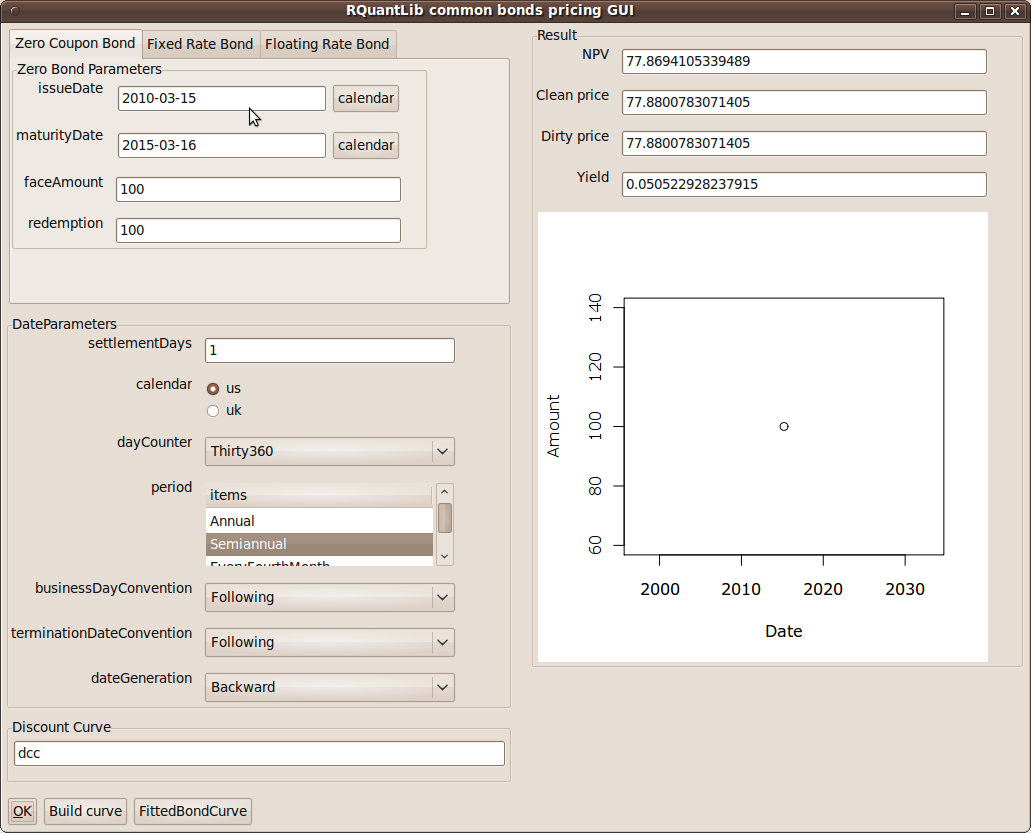
\includegraphics{figures/bondGUI.png}}
\end{center}
\end{frame}


\end{document}

%%% Local Variables: 
%%% mode: latex
%%% TeX-master: t
%%% End: 
